\documentclass{article}
\usepackage{minted}
\usepackage{cleveref}
\usepackage{graphicx}
\usepackage{listings}
\usepackage{courier}
\usepackage[backend=biber,citestyle=authoryear,url=true,backref=bibtex,bibstyle=apa,useprefix=true]{biblatex}
\setminted[java]{fontfamily=courier}

\addbibresource{bibliography.bib}
\begin{document}
	\section{Source code}\label{sec:code} % (fold)
	The source code of this application, in its entirety can be found below, split up as follows: 
	\begin{itemize}
		\item Main source code 
		\item Facilities
		\item Exceptions
		\item Comparators
	\end{itemize}

	\subsection{Main source code}\label{sub:main_source_code} % (fold)
	\textit{MedicalConsole.java}
	\inputminted{java}{src/main/java/com/yvesstraten/medicalconsole/MedicalConsole.java}

	\textit{Format.java}
	\inputminted{java}{src/main/java/com/yvesstraten/medicalconsole/Format.java}

	\textit{Input.java}
	\inputminted{java}{src/main/java/com/yvesstraten/medicalconsole/Input.java}

	\textit{ArrayListSet.java}
	\inputminted{java}{./src/main/java/com/yvesstraten/medicalconsole/ArrayListSet.java}

	\newpage 

	\textit{Editable.java}\label{Editable}
	\inputminted{java}{src/main/java/com/yvesstraten/medicalconsole/Editable.java}

	\textit{HealthService.java}
	\inputminted{java}{src/main/java/com/yvesstraten/medicalconsole/HealthService.java}

	\textit{IdGenerator.java}
	\inputminted{java}{src/main/java/com/yvesstraten/medicalconsole/IdGenerator.java}
	% subsection Main source code (end)

	\subsection{Facilities}\label{sub:facilities} % (fold)
	\textit{Clinic.java}
	\inputminted{java}{src/main/java/com/yvesstraten/medicalconsole/facilities/Clinic.java}

	\textit{Hospital.java}
	\inputminted{java}{src/main/java/com/yvesstraten/medicalconsole/facilities/Hospital.java}

	\textit{MedicalFacility.java}
	\inputminted{java}{src/main/java/com/yvesstraten/medicalconsole/facilities/MedicalFacility.java}

	\textit{Procedure.java}
	\inputminted{java}{src/main/java/com/yvesstraten/medicalconsole/facilities/Procedure.java}

	\textit{Patient.java}
	\inputminted{java}{src/main/java/com/yvesstraten/medicalconsole/Patient.java}
	% subsection Facilities (end)

	\subsection{Comparators}\label{sub:comparators} % (fold)
	\textit{MedicalFacilitiesComparators.java}
	\inputminted{java}{src/main/java/com/yvesstraten/medicalconsole/comparators/MedicalFacilitiesComparators.java}

	\textit{PatientComparators.java}
	\inputminted{java}{src/main/java/com/yvesstraten/medicalconsole/comparators/PatientComparators.java}

	\textit{ProcedureComparators.java}
	\inputminted{java}{src/main/java/com/yvesstraten/medicalconsole/comparators/ProcedureComparators.java}
	% subsection Comparators (end)

  \newpage

	\subsection{Exceptions}\label{sub:exceptions} % (fold)
	\textit{ClassIsNotEditableException.java}
	\inputminted{java}{src/main/java/com/yvesstraten/medicalconsole/exceptions/ClassIsNotEditableException.java}

	\textit{InvalidOptionException.java}
	\inputminted{java}{src/main/java/com/yvesstraten/medicalconsole/exceptions/InvalidOptionException.java}

	\textit{InvalidYesNoException.java}
	\inputminted{java}{src/main/java/com/yvesstraten/medicalconsole/exceptions/InvalidYesNoException.java}

	\textit{NegativeNumberException.java}
	\inputminted{java}{src/main/java/com/yvesstraten/medicalconsole/exceptions/NegativeNumberException.java}

	\textit{NoHospitalsAvailableException.java}
	\inputminted{java}{src/main/java/com/yvesstraten/medicalconsole/exceptions/NoHospitalsAvailableException.java}

	\textit{WrongHospitalException.java}
	\inputminted{java}{src/main/java/com/yvesstraten/medicalconsole/exceptions/WrongHospitalException.java}
	% subsection Exceptions (end)

	\section{Unit tests}\label{sec:unit_tests} % (fold)
	For this assignment, unit tests written in JUNIT 5 \textcite{Junit5} were used extensively. Each unit test is show as follows:
	
	\textit{AddTests.java} 
	\inputminted{java}{src/test/java/com/yvesstraten/medicalconsole/tests/AddTests.java}

	\textit{ClinicTests.java} 
	\inputminted{java}{src/test/java/com/yvesstraten/medicalconsole/tests/ClinicTests.java}

	\textit{DeleteTests.java} 
	\inputminted{java}{src/test/java/com/yvesstraten/medicalconsole/tests/DeleteTests.java}

	\textit{EditTests.java}\label{Edit_tests} 
	\inputminted{java}{src/test/java/com/yvesstraten/medicalconsole/tests/EditTests.java}

	\textit{FacilitiesTests.java} 
	\inputminted{java}{src/test/java/com/yvesstraten/medicalconsole/tests/FacilitiesTests.java}

	\textit{FormatTests.java} 
	\inputminted{java}{src/test/java/com/yvesstraten/medicalconsole/tests/FormatTests.java}

	\textit{HealthServiceTests.java} 
	\inputminted{java}{src/test/java/com/yvesstraten/medicalconsole/tests/HealthServiceTests.java}

	\textit{HospitalTests.java} 
	\inputminted{java}{src/test/java/com/yvesstraten/medicalconsole/tests/HospitalTests.java}

	\textit{MedicalConsoleTest.java} 
	\inputminted{java}{src/test/java/com/yvesstraten/medicalconsole/tests/MedicalConsoleTest.java}

	\textit{MedicalConsoleTests.java} 
	\inputminted{java}{src/test/java/com/yvesstraten/medicalconsole/tests/MedicalConsoleTests.java}

	\textit{PatientTests.java} 
	\inputminted{java}{src/test/java/com/yvesstraten/medicalconsole/tests/PatientTests.java}

	\textit{ProcedureTests.java} 
	\inputminted{java}{src/test/java/com/yvesstraten/medicalconsole/tests/ProcedureTests.java}

	\textit{SortingTest.java}\label{sorting_tests} 
	\inputminted{java}{src/test/java/com/yvesstraten/medicalconsole/tests/SortingTest.java}

	When running these tests with \textit{mvn test} the following output is shown:
	\begin{figure}
		\begin{center}
			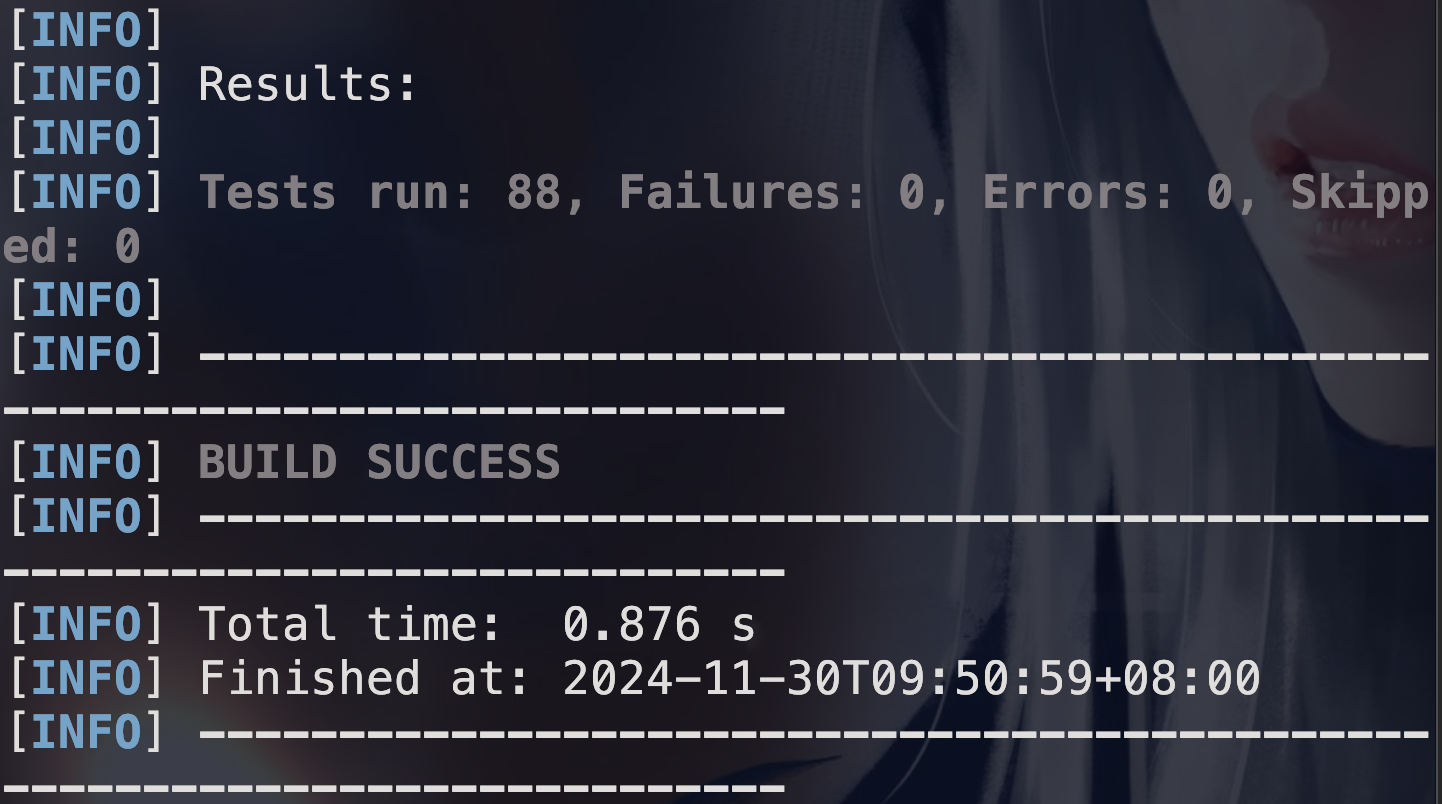
\includegraphics[width=0.8\textwidth]{figures/Mvn_test.png}
		\end{center}
		\caption{Test output}\label{fig:}
	\end{figure}
	
	% section Unit tests (end)

	\newpage

	\section{Core runtime output}\label{sec:runtime_output} % (fold)
	Several runtime tests have been undertaken as well to test core functions of the program. These are:
	\begin{itemize}
		\item Adding objects
		\item Listing objects
		\item Deleting objects
		\item Simulate a visit
		\item Operate on a patient
	\end{itemize}

	\subsection{Adding objects}\label{sub:adding_objects} % (fold)
	In this test, addition of objects will be tested with random misinputs to also check for the robustness of the system. The tests are undertaken in the following order: 
	\begin{itemize}
		\item Clinic 
		\item Hospital 
		\item Patient
		\item Procedure
	\end{itemize}

	\textit{Clinic}
	\begin{figure}
		\begin{center}
			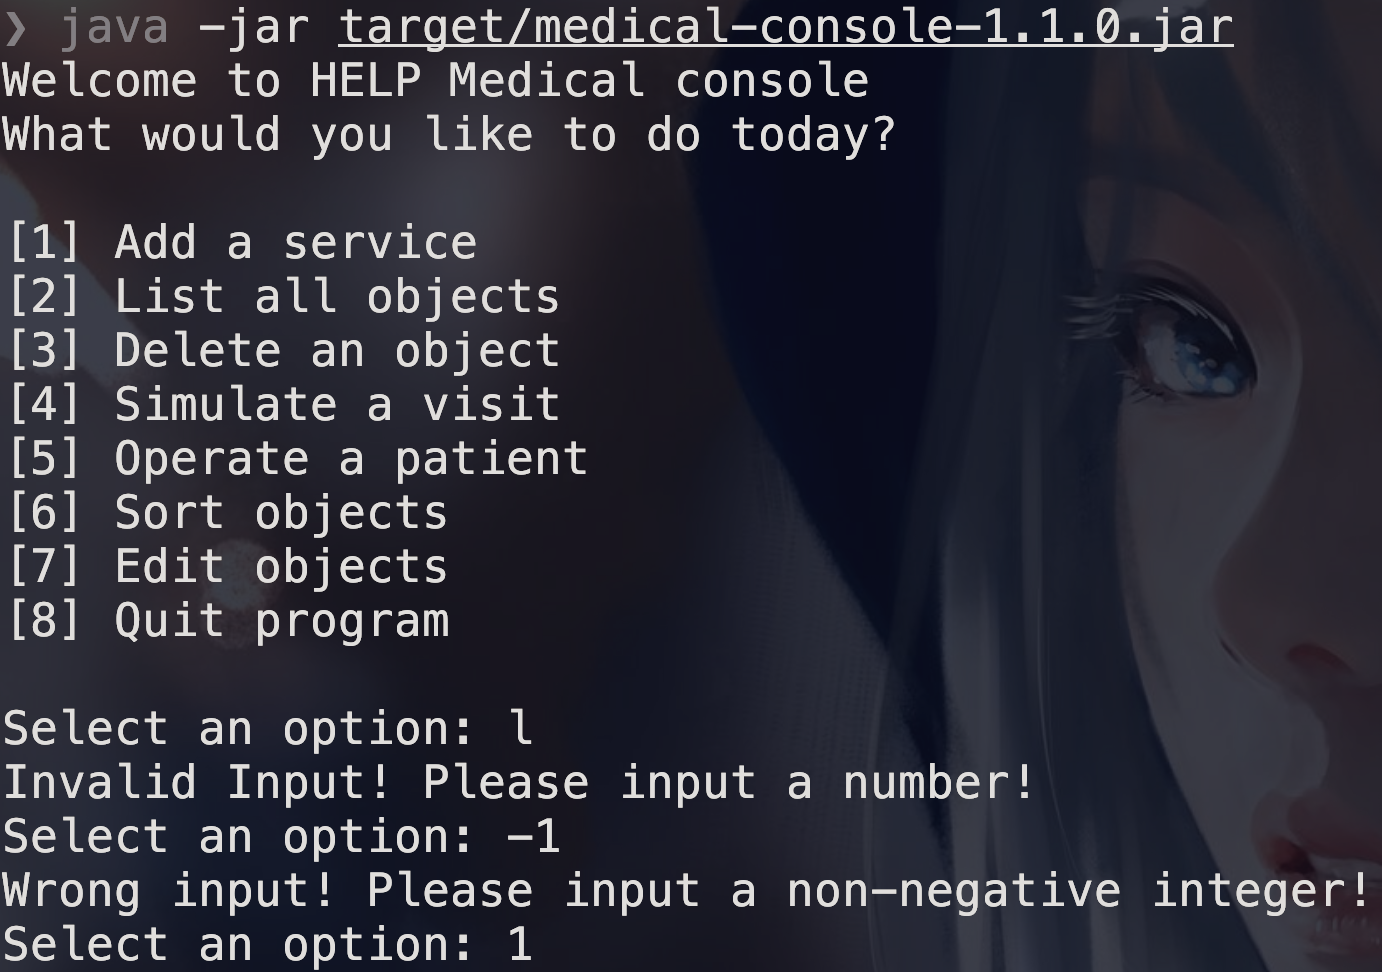
\includegraphics[width=0.7\textwidth]{figures/Adding/Clinic/Clinic_01.png}
		\end{center}
		\caption{Getting to the addition menu}\label{fig:clinic_01}
	\end{figure}

	\begin{figure}
		\begin{center}
			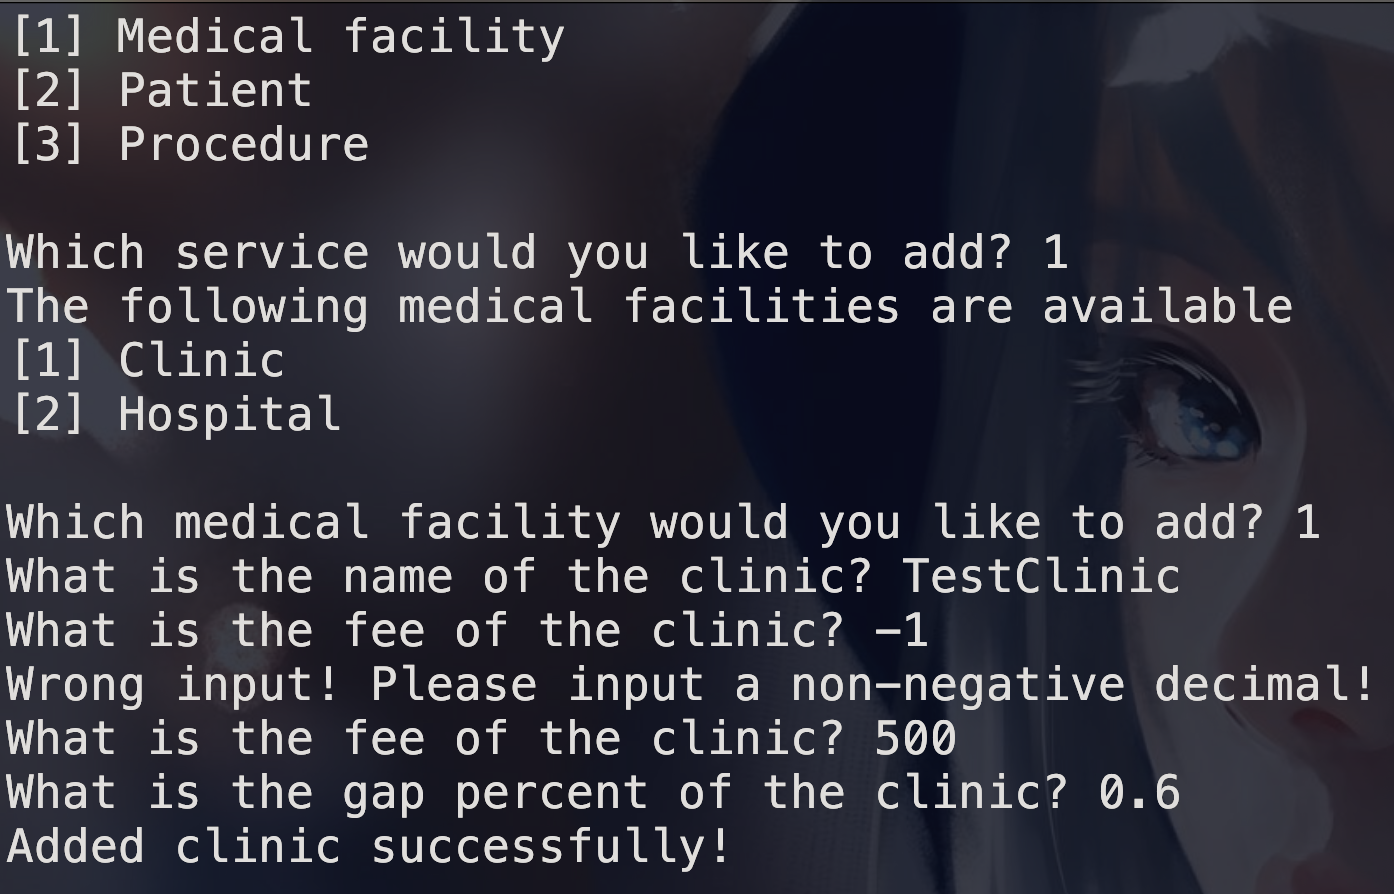
\includegraphics[width=0.7\textwidth]{figures/Adding/Clinic/Clinic_02.png}
		\end{center}
		\caption{Adding clinic}\label{fig:clinic_02}
	\end{figure}

	\textit{Hospital}
	\begin{figure}
		\begin{center}
			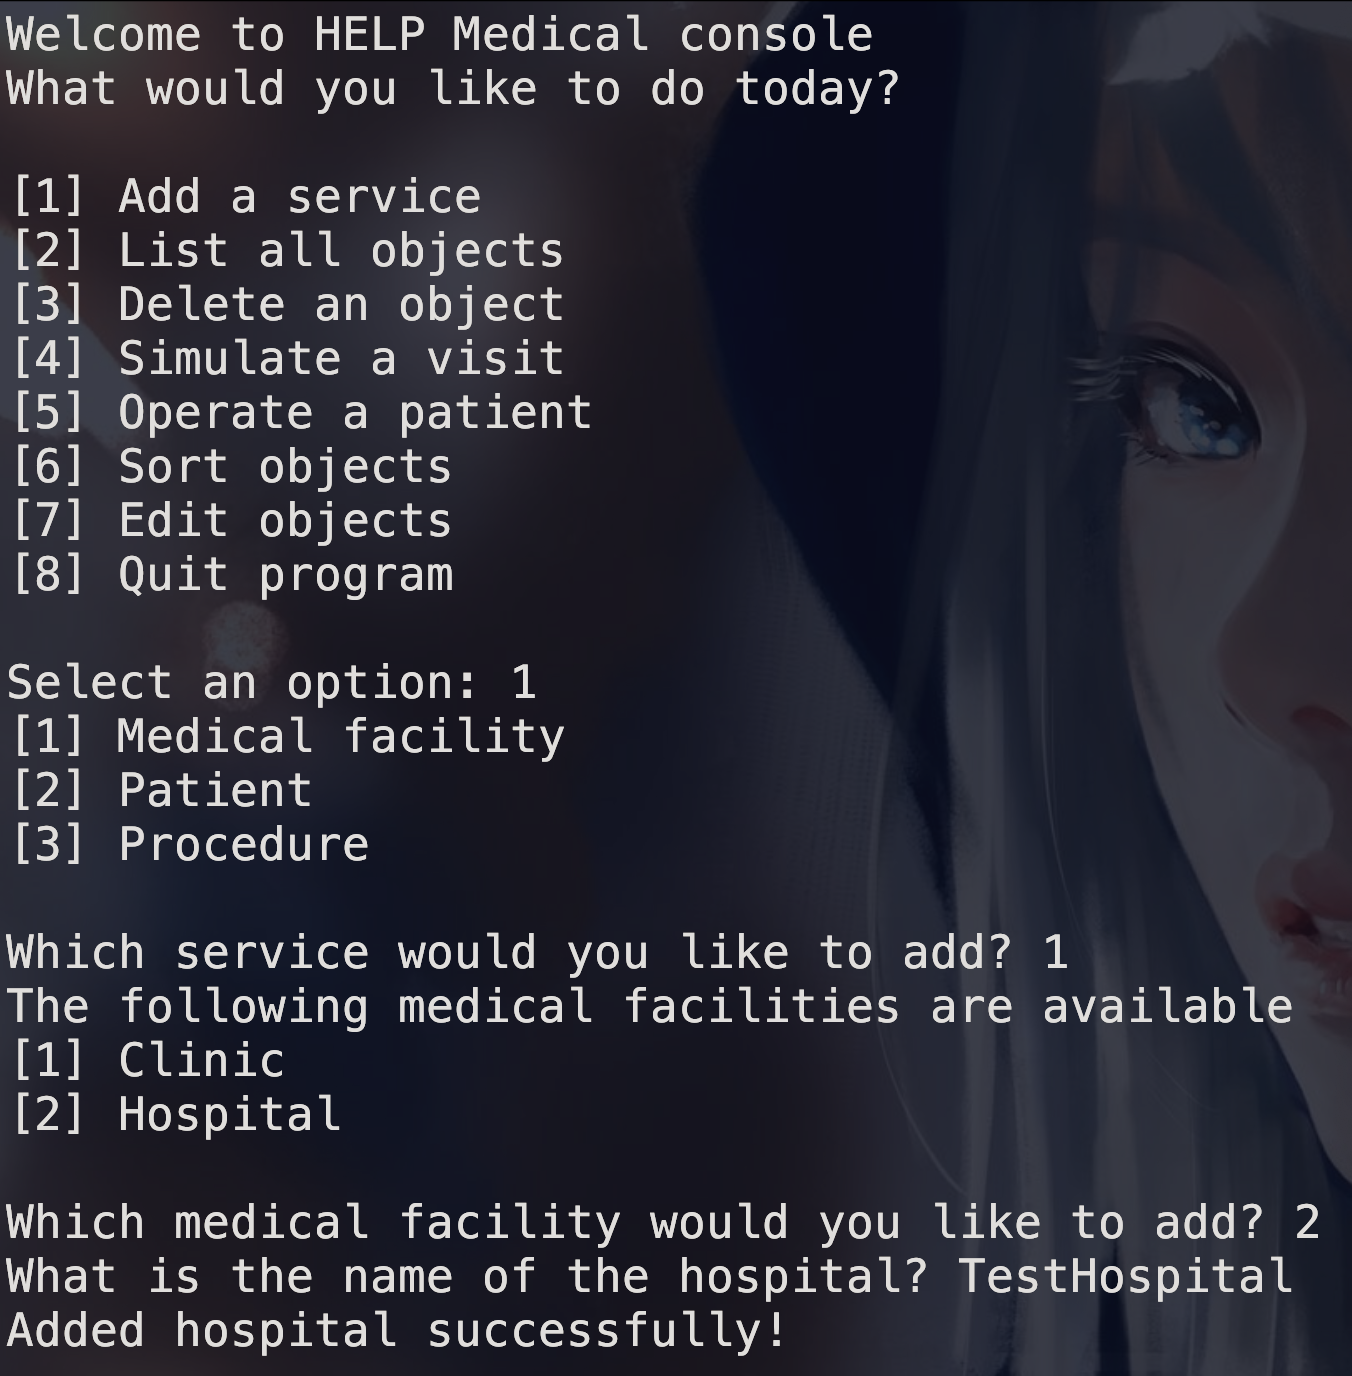
\includegraphics[width=0.5\textwidth]{figures/Adding/Hospital/Hospital_01.png}
		\end{center}
		\caption{Adding a hospital}\label{fig:hospital_01}
	\end{figure}

	\newpage

	\textit{Patient}
	\begin{figure}
		\begin{center}
			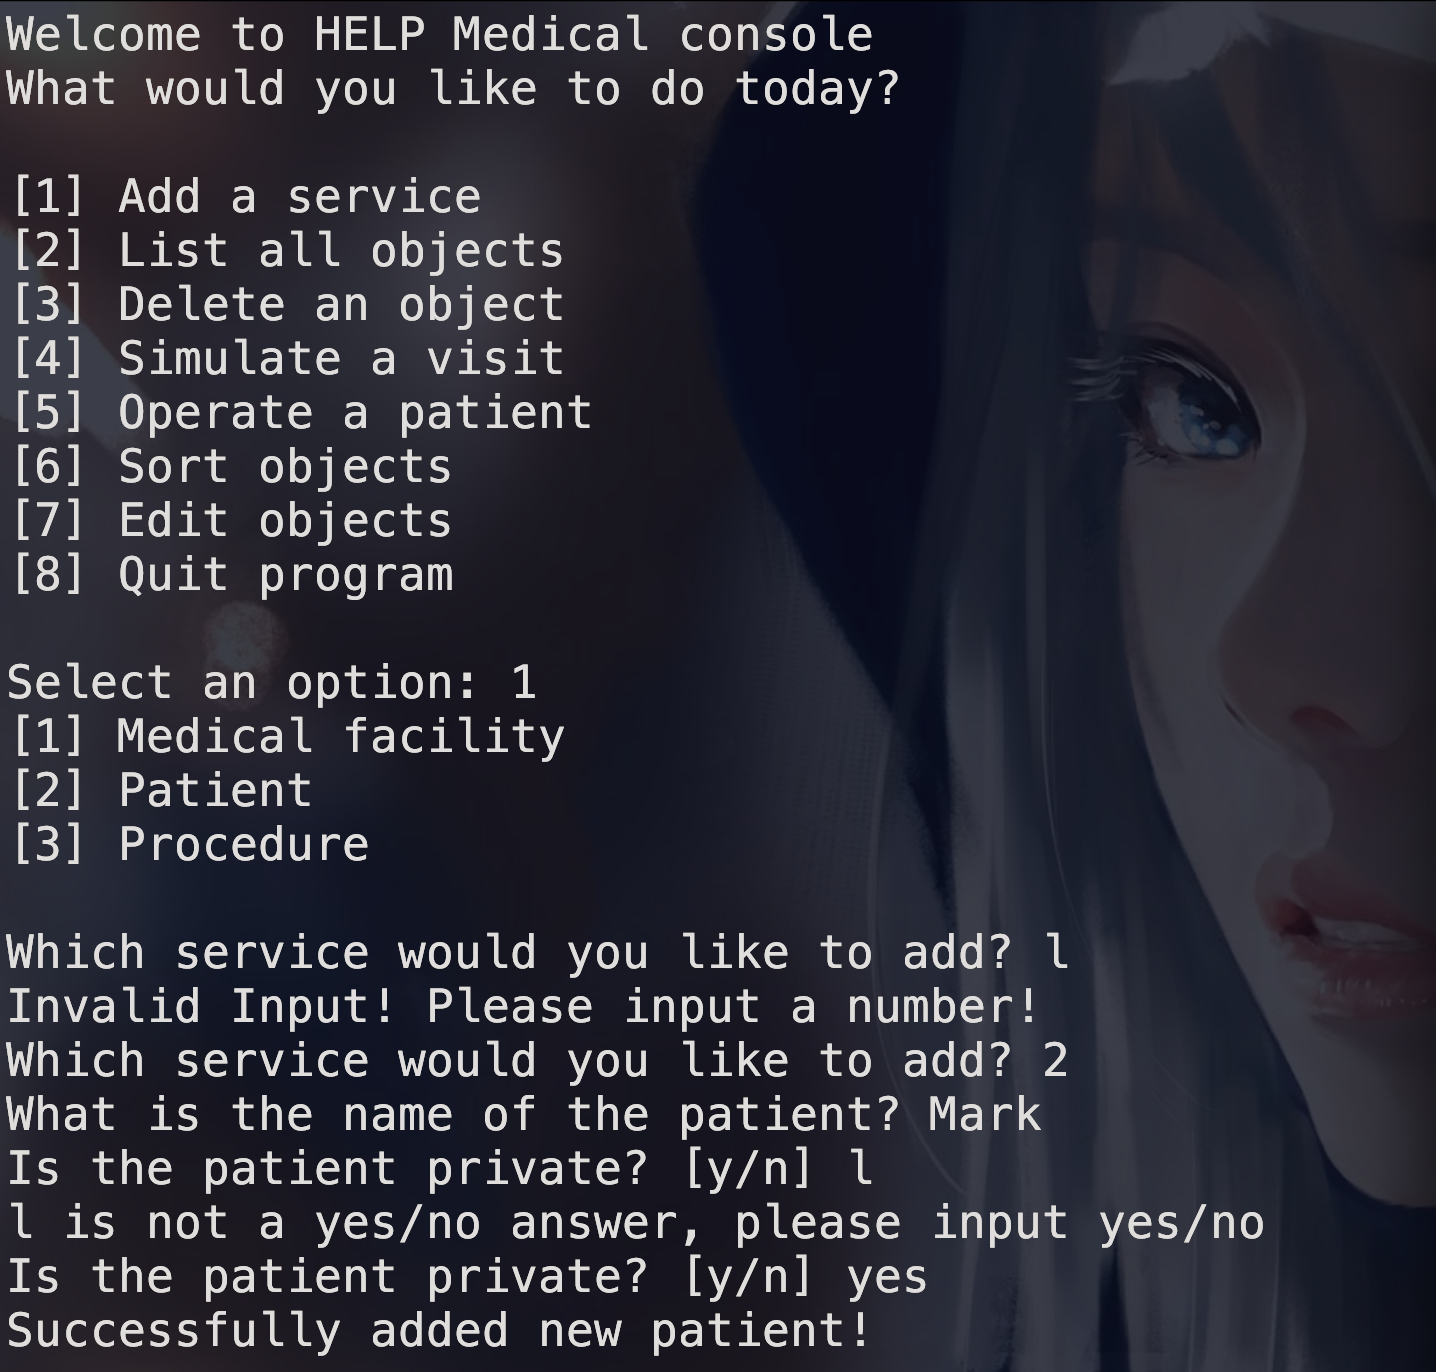
\includegraphics[width=0.5\textwidth]{figures/Adding/Patient/Patient_01.png}
		\end{center}
		\caption{Adding a patient}\label{fig:patient_01}
	\end{figure}

	\textit{Procedure}
	\begin{figure}
		\begin{center}
			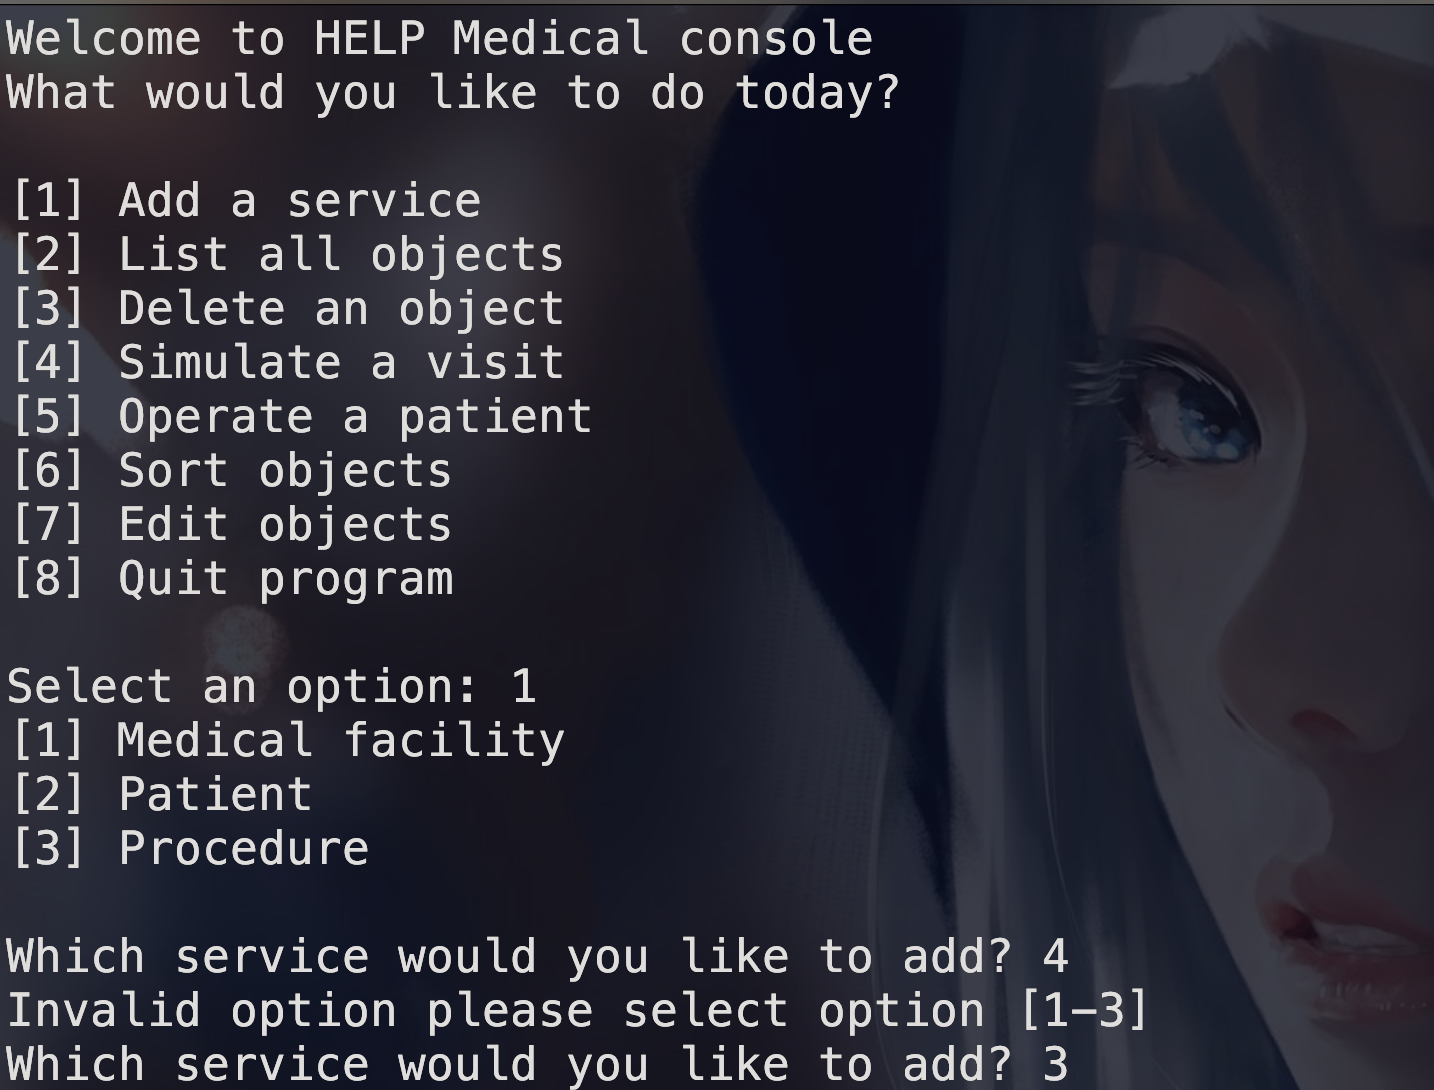
\includegraphics[width=0.7\textwidth]{figures/Adding/Procedure/Procedure_01.png}
		\end{center}
		\caption{Getting to the procedure menu}\label{fig:procedure_01}
	\end{figure}
	
	\begin{figure}
		\begin{center}
			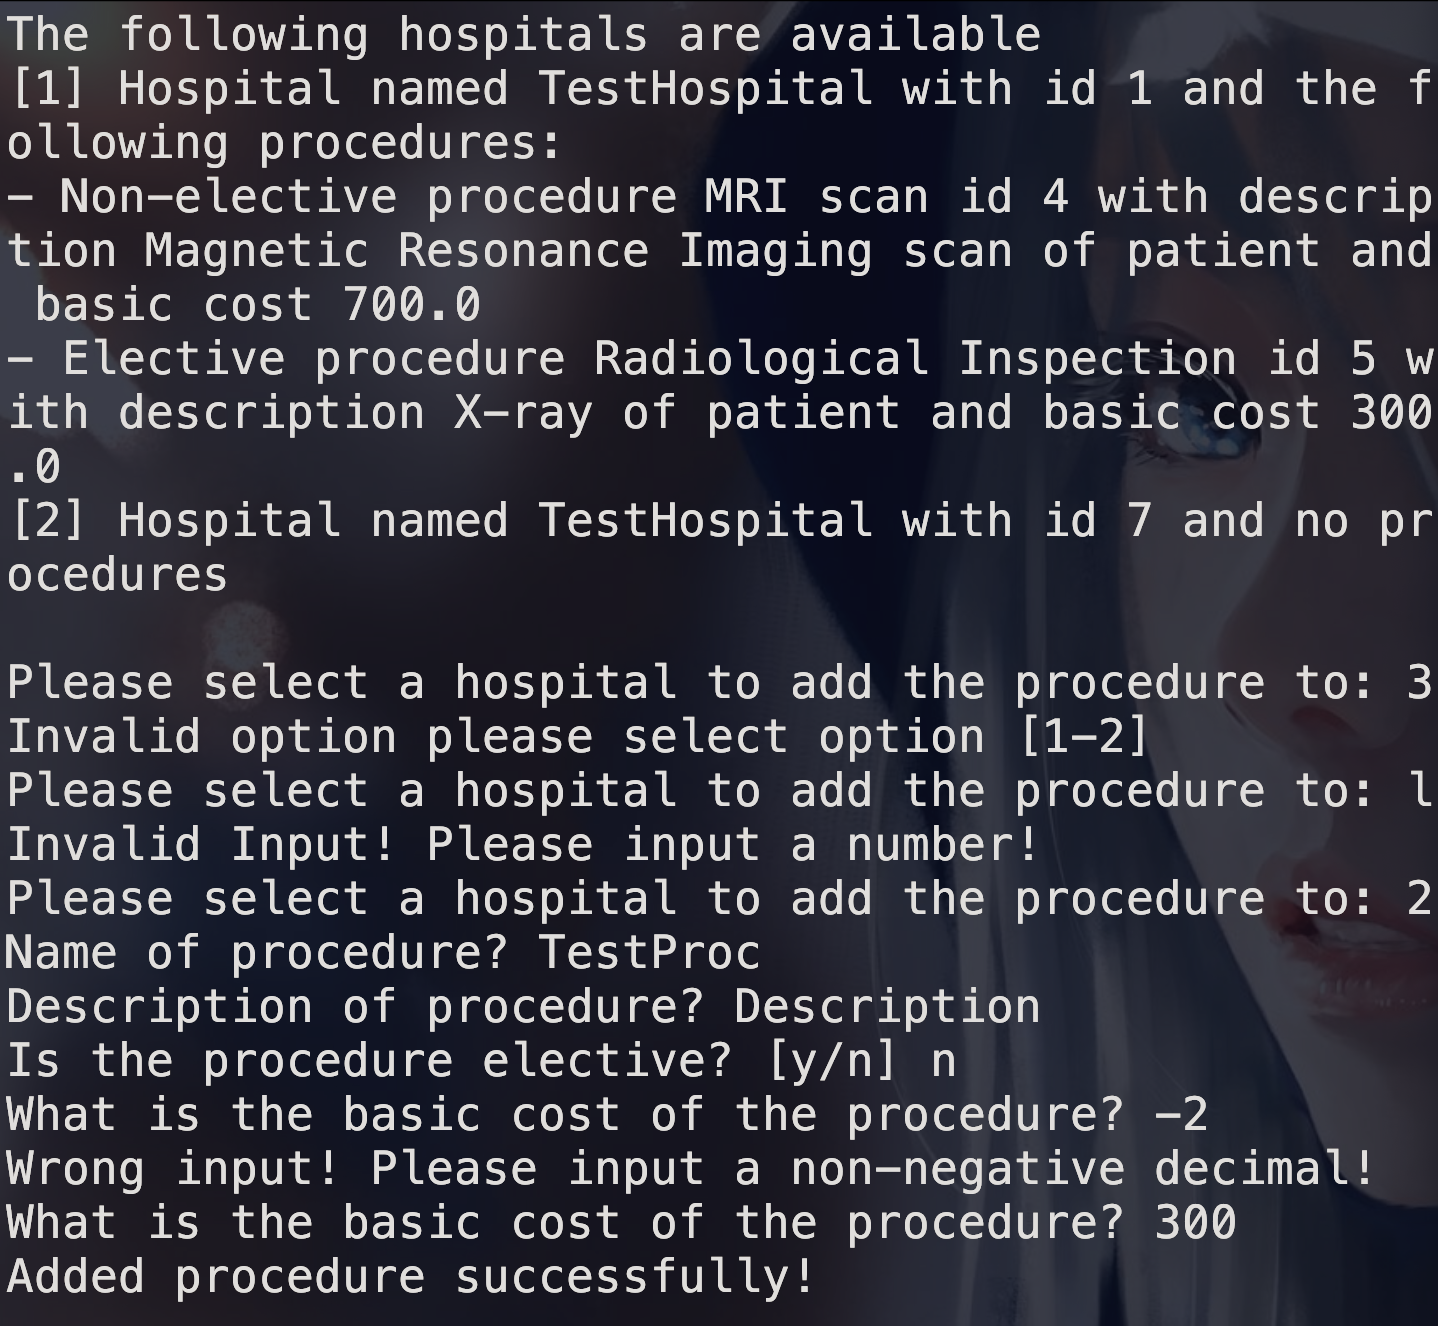
\includegraphics[width=0.7\textwidth]{figures/Adding/Procedure/Procedure_02.png}
		\end{center}
		\caption{Adding a procedure}\label{fig:procedure_02}
	\end{figure}

	As you can see, objects can be freely added, and each input is checked for validity. Furthermore, each input can be repeated on error, without sending the user back to the main menu each time.
	% subsection Adding objects (end)

	\newpage 

	\subsection{Listing objects}\label{sub:listing_objects} % (fold)
	In this test, the listing of objects will be tested in the same way as addition testing. This run is done immediately after the addition of these test objects.

	\newpage 

	\textit{Medical facilities}
	\begin{figure}
		\begin{center}
			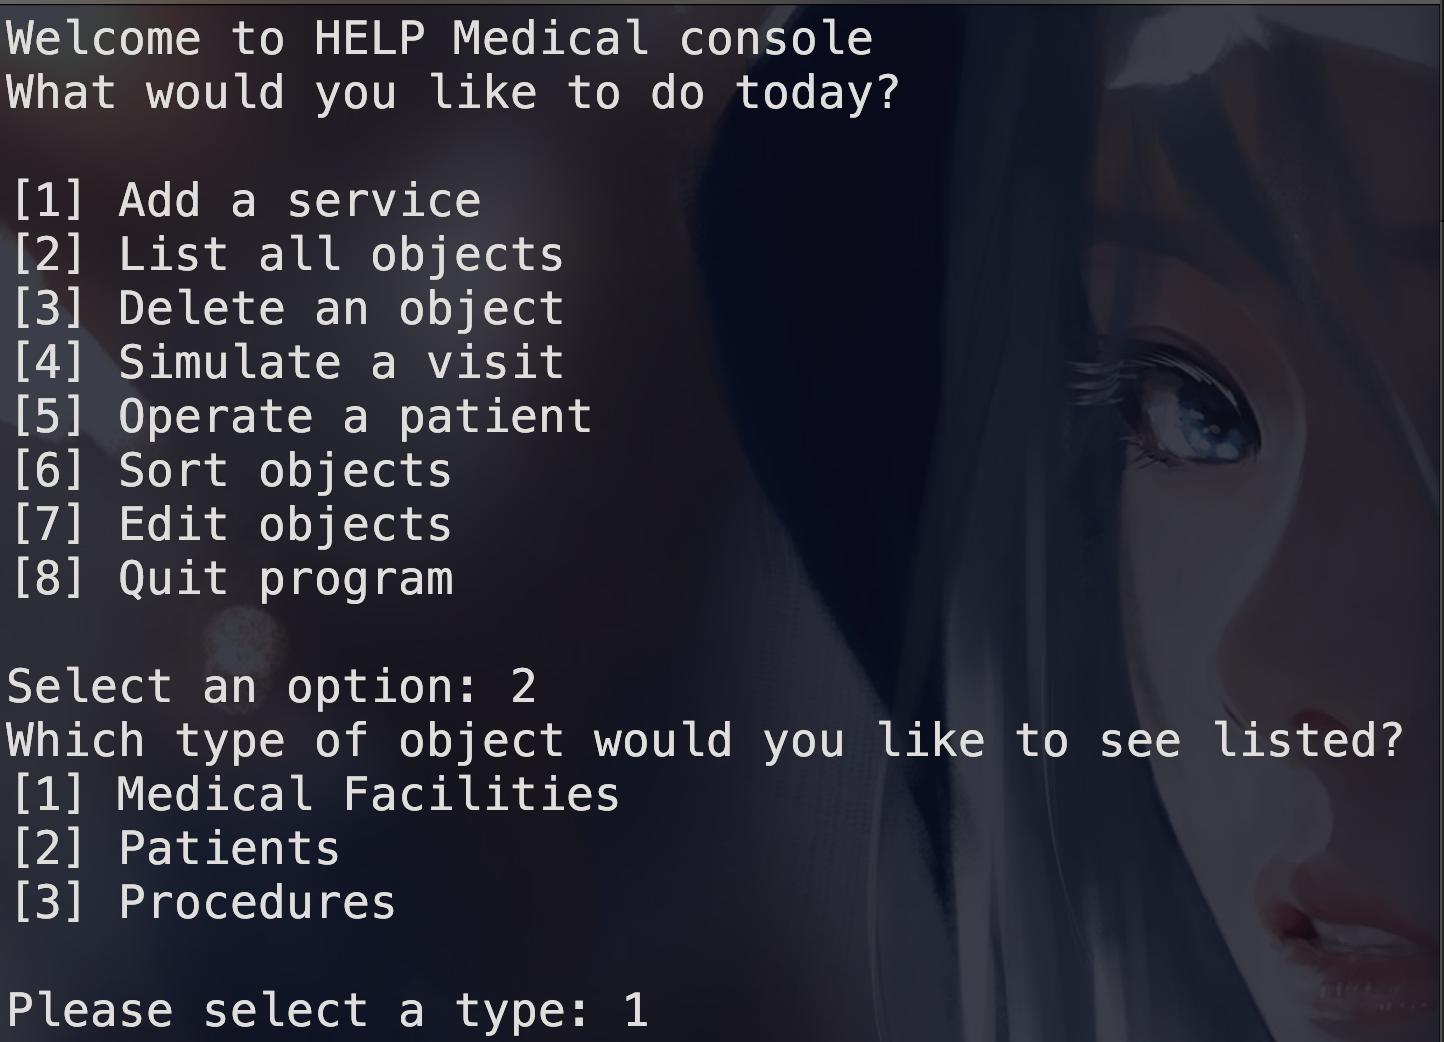
\includegraphics[width=0.7\textwidth]{figures/Listing/Listing_Medical_01.png}
		\end{center}
		\caption{Getting to the Medical List menu}\label{fig:listing_medical_01}
	\end{figure}
	
	\begin{figure}
		\begin{center}
			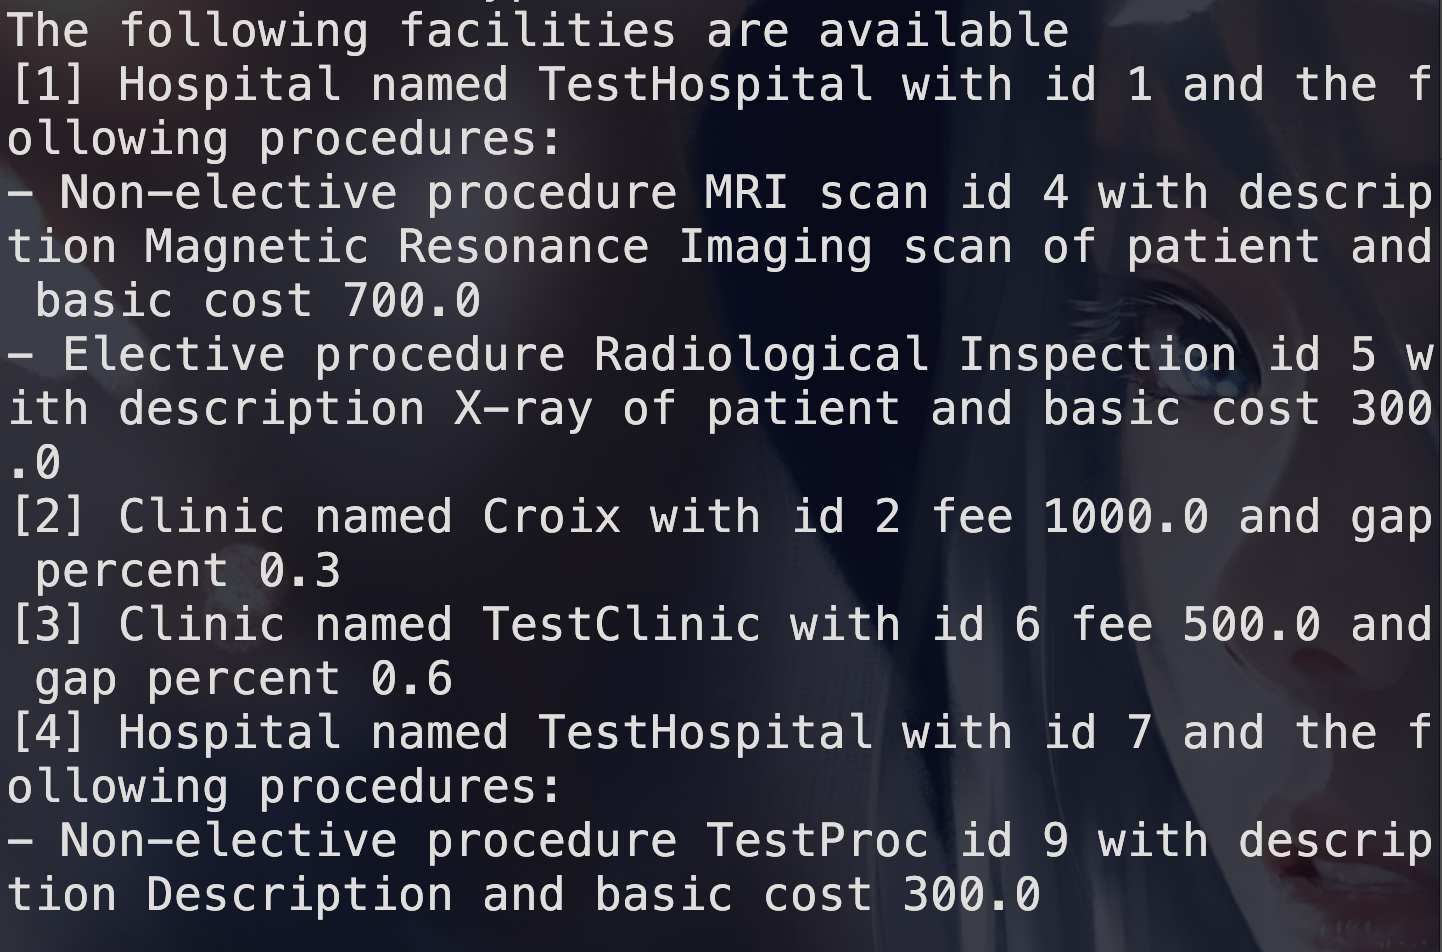
\includegraphics[width=0.7\textwidth]{figures/Listing/Listing_Medical_02.png}
		\end{center}
		\caption{Listing medical facilities}\label{fig:listing_medical_02}
	\end{figure}
	
	\textit{Patients}
	\begin{figure}
		\begin{center}
			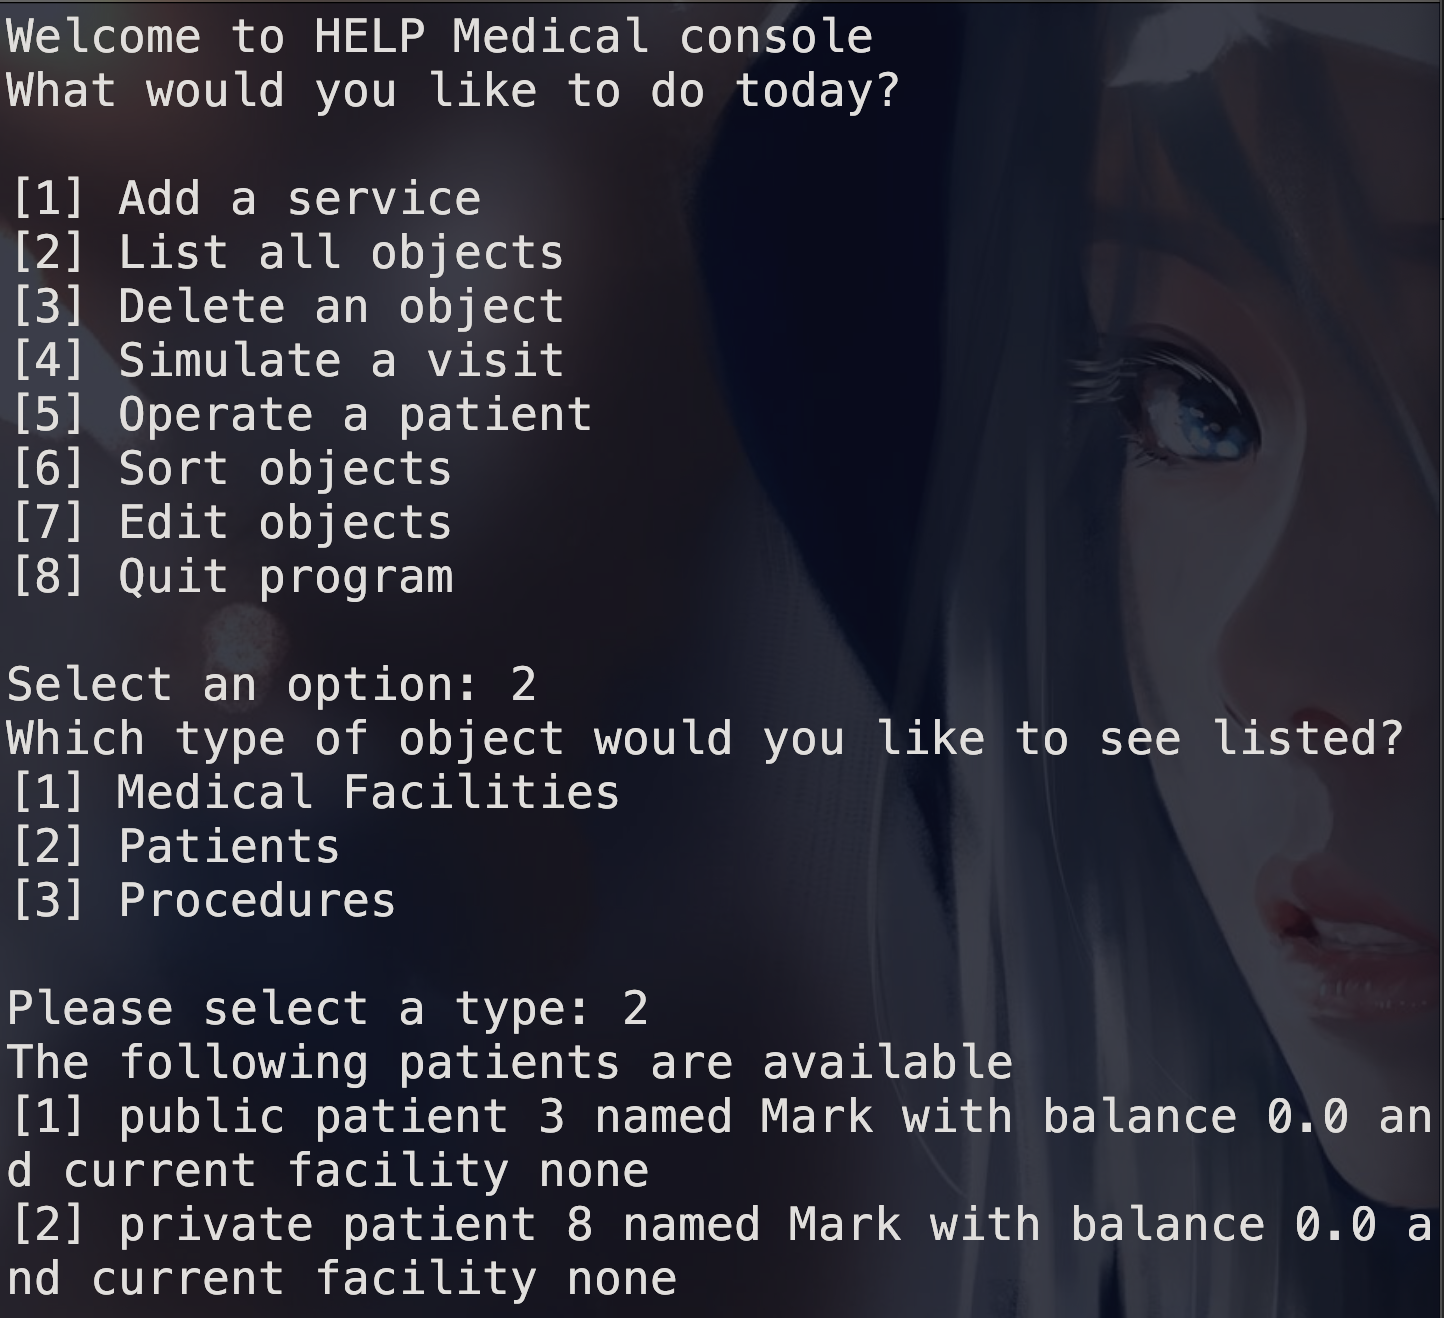
\includegraphics[width=0.7\textwidth]{figures/Listing/Listing_Patients.png}
		\end{center}
		\caption{Listing patients}\label{fig:listing_patients}
	\end{figure}
	
	\textit{Procedures}
	\begin{figure}
		\begin{center}
			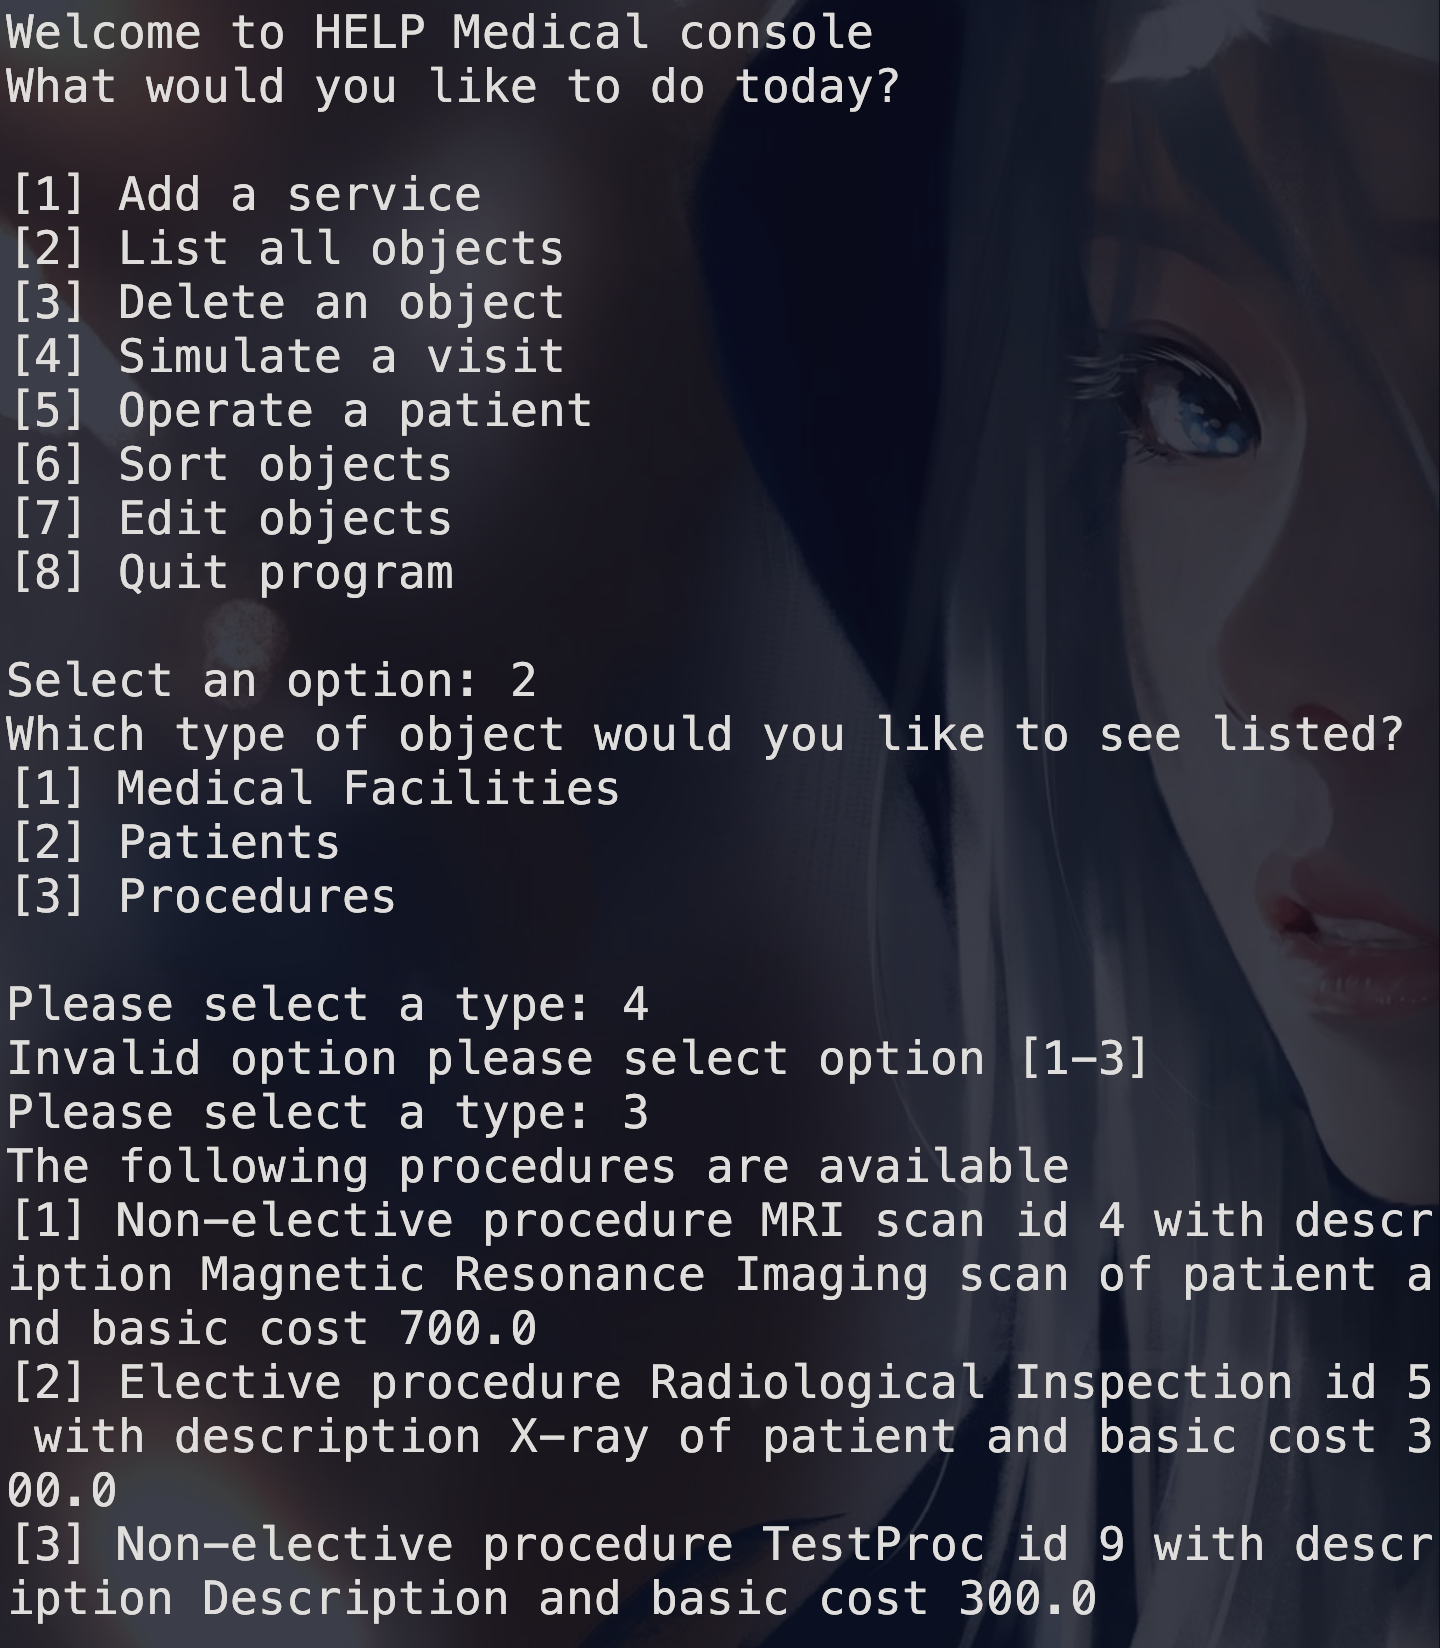
\includegraphics[width=0.7\textwidth]{figures/Listing/Listing_Procedures.png}
		\end{center}
		\caption{Listing procedures}\label{fig:listing_procedures}
	\end{figure}
	% subsection Listing objects (end)

	\subsection{Deleting objects}\label{sub:deleting_objects} % (fold)
	In this test, the listing of objects will be tested in the same way as addition testing. This run is done immediately after the addition of these test objects.

	\textit{Hospital}
	\begin{figure}
		\begin{center}
			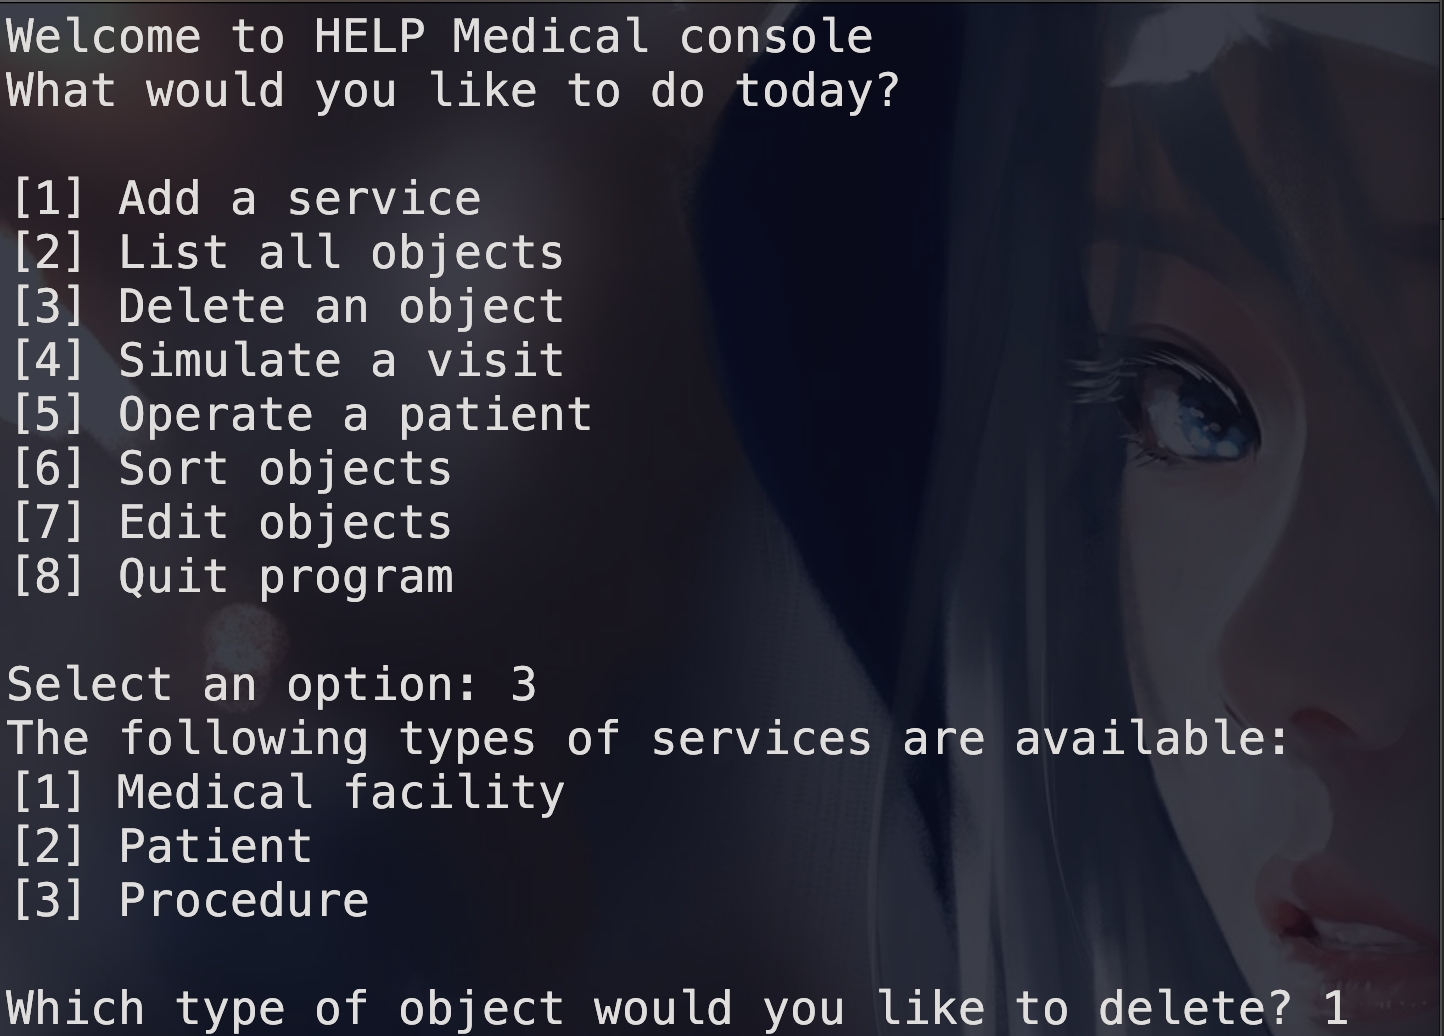
\includegraphics[width=0.6\textwidth]{figures/Deleting/Deleting_Hospital_01.png}
		\end{center}
		\caption{Getting to the facility deletion menu}\label{fig:deleting_hospital_01}
	\end{figure}
	
	\begin{figure}
		\begin{center}
			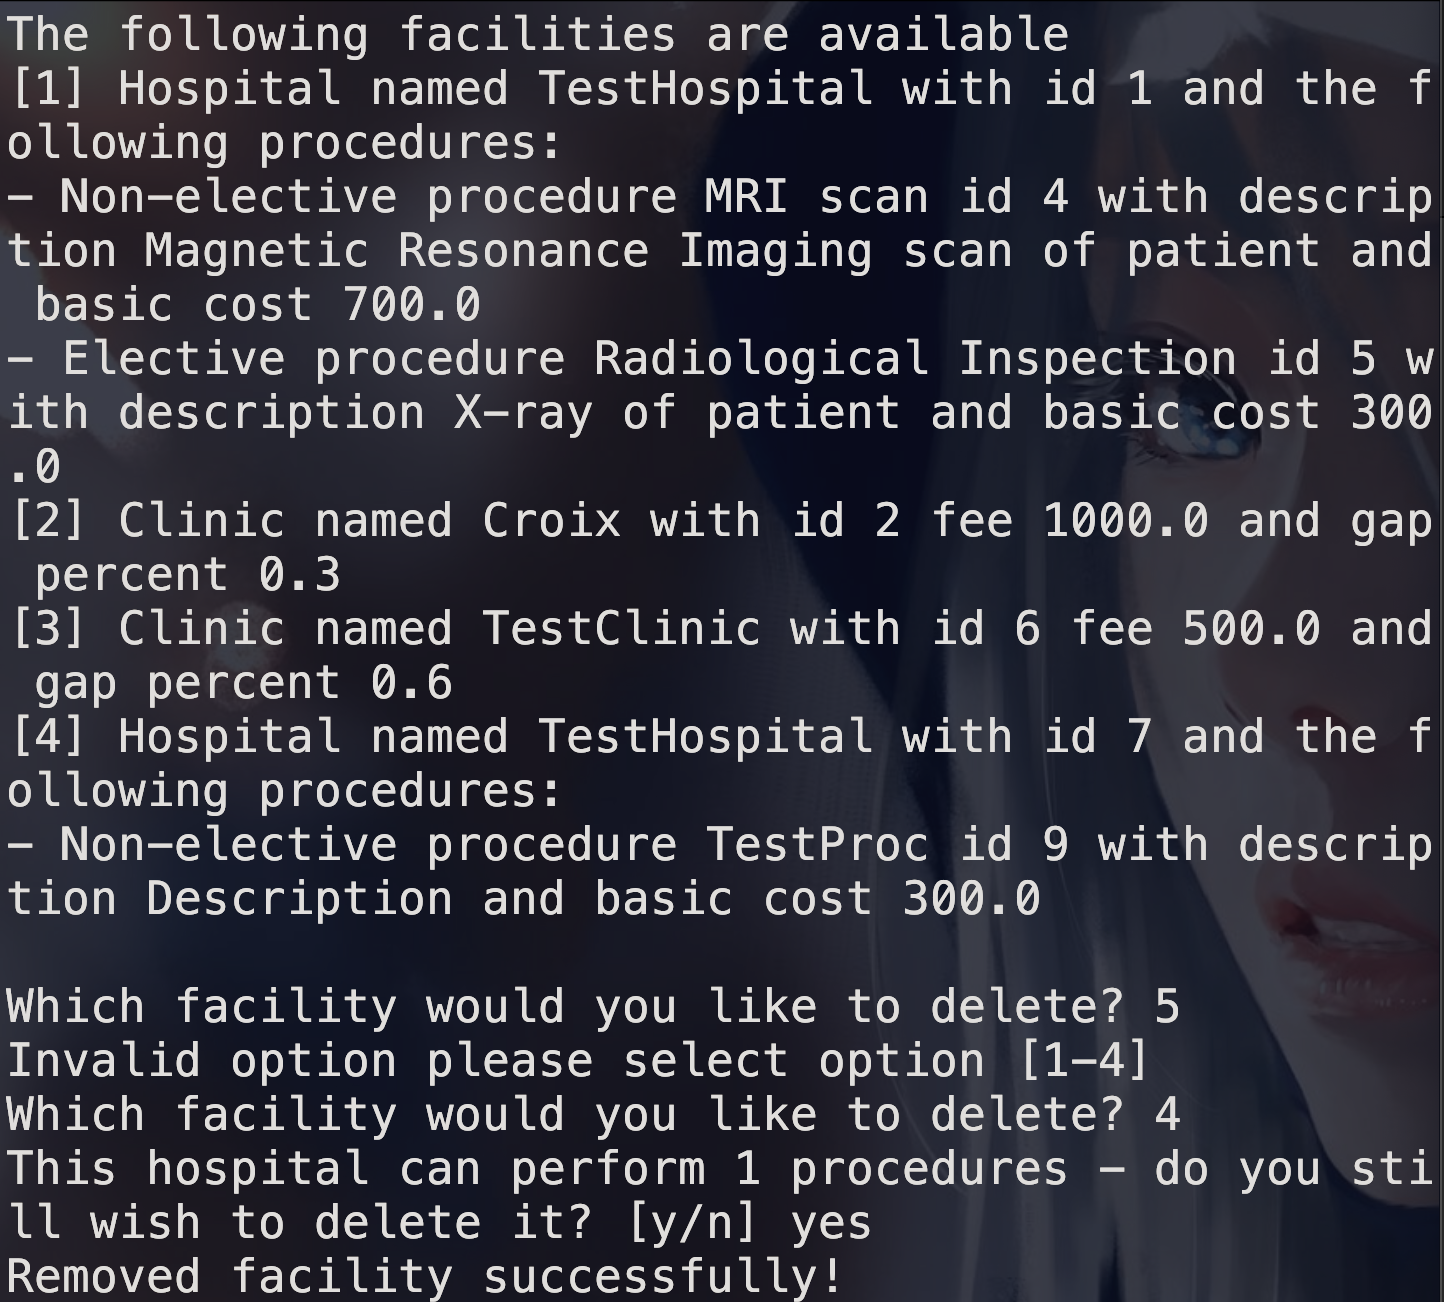
\includegraphics[width=0.6\textwidth]{figures/Deleting/Deleting_Hospital_02.png}
		\end{center}
		\caption{Deleting hospital with procedures}\label{fig:deleting_hospital_02}
	\end{figure}
	
	\textit{Clinic}
	\begin{figure}
		\begin{center}
			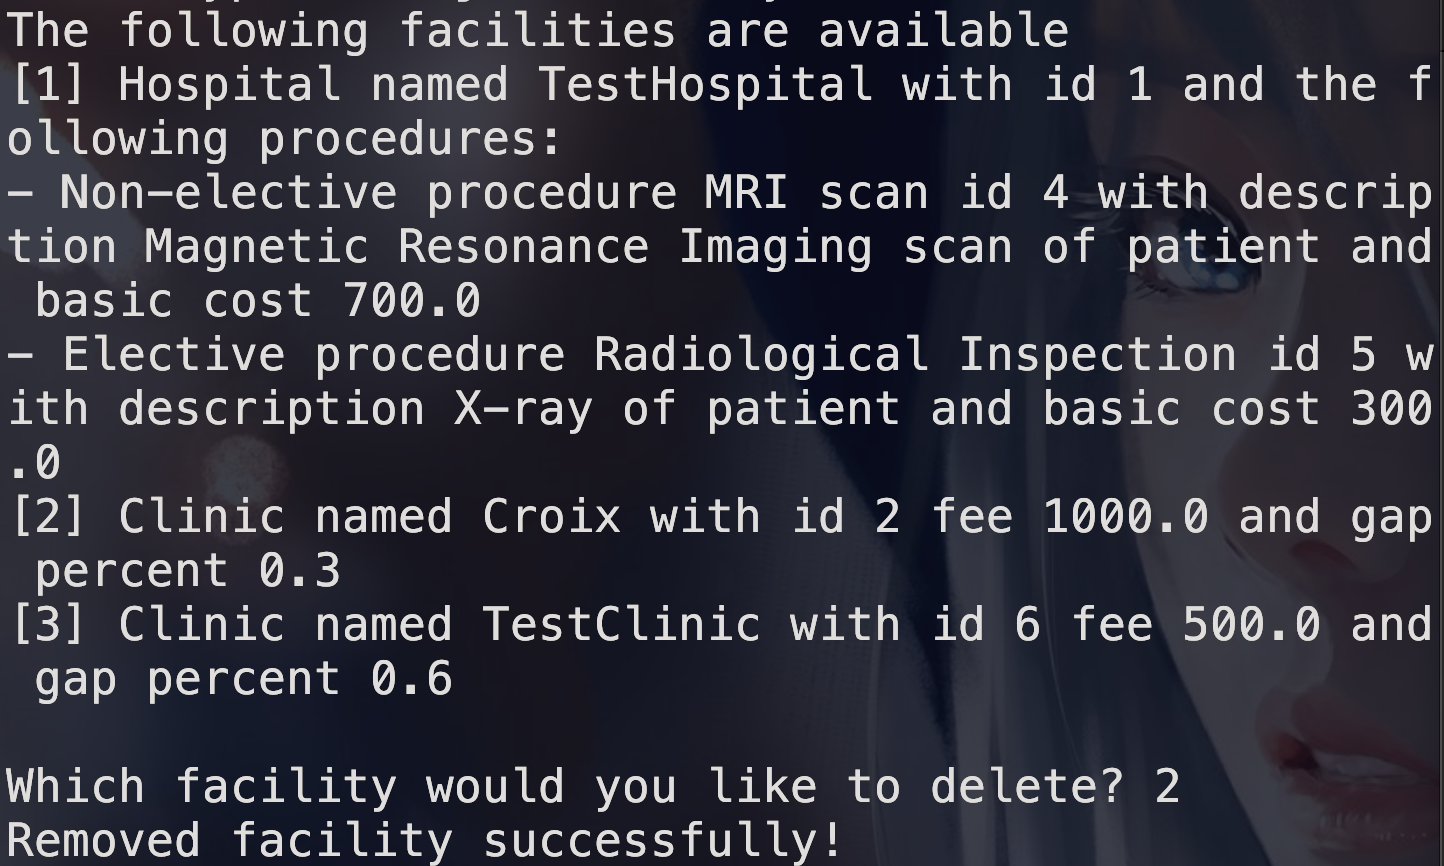
\includegraphics[width=0.6\textwidth]{figures/Deleting/Deleting_Clinic_02.png}
		\end{center}
		\caption{Deleting clinic}\label{fig:deleting_clinic_02}
	\end{figure}
	
	\textit{Patient}
	\begin{figure}
		\begin{center}
			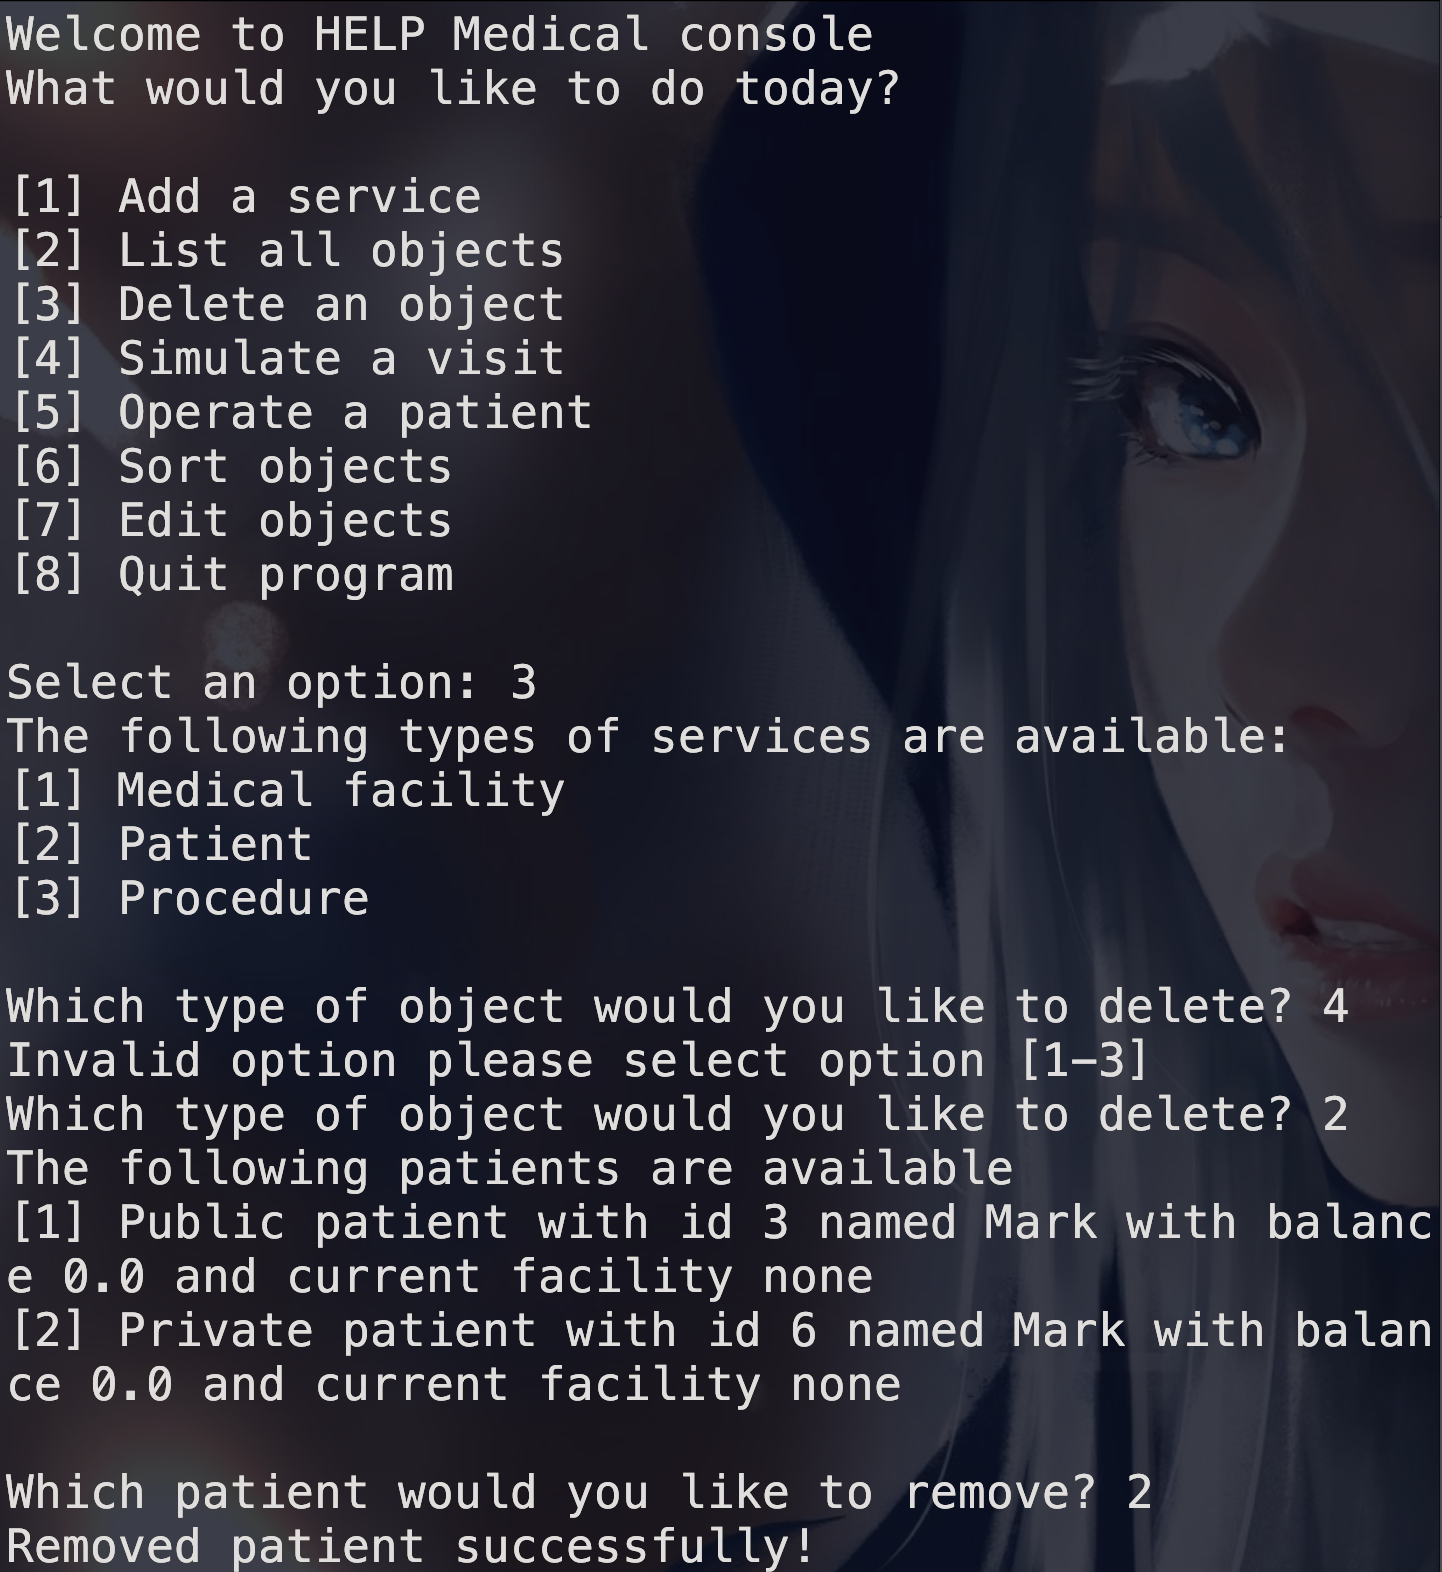
\includegraphics[width=0.6\textwidth]{figures/Deleting/Deleting_Patient_01.png}
		\end{center}
		\caption{Deleting Patient}\label{fig:deleting_patient_01}
	\end{figure}

	\textit{Procedure}
	\begin{figure}
		\begin{center}
			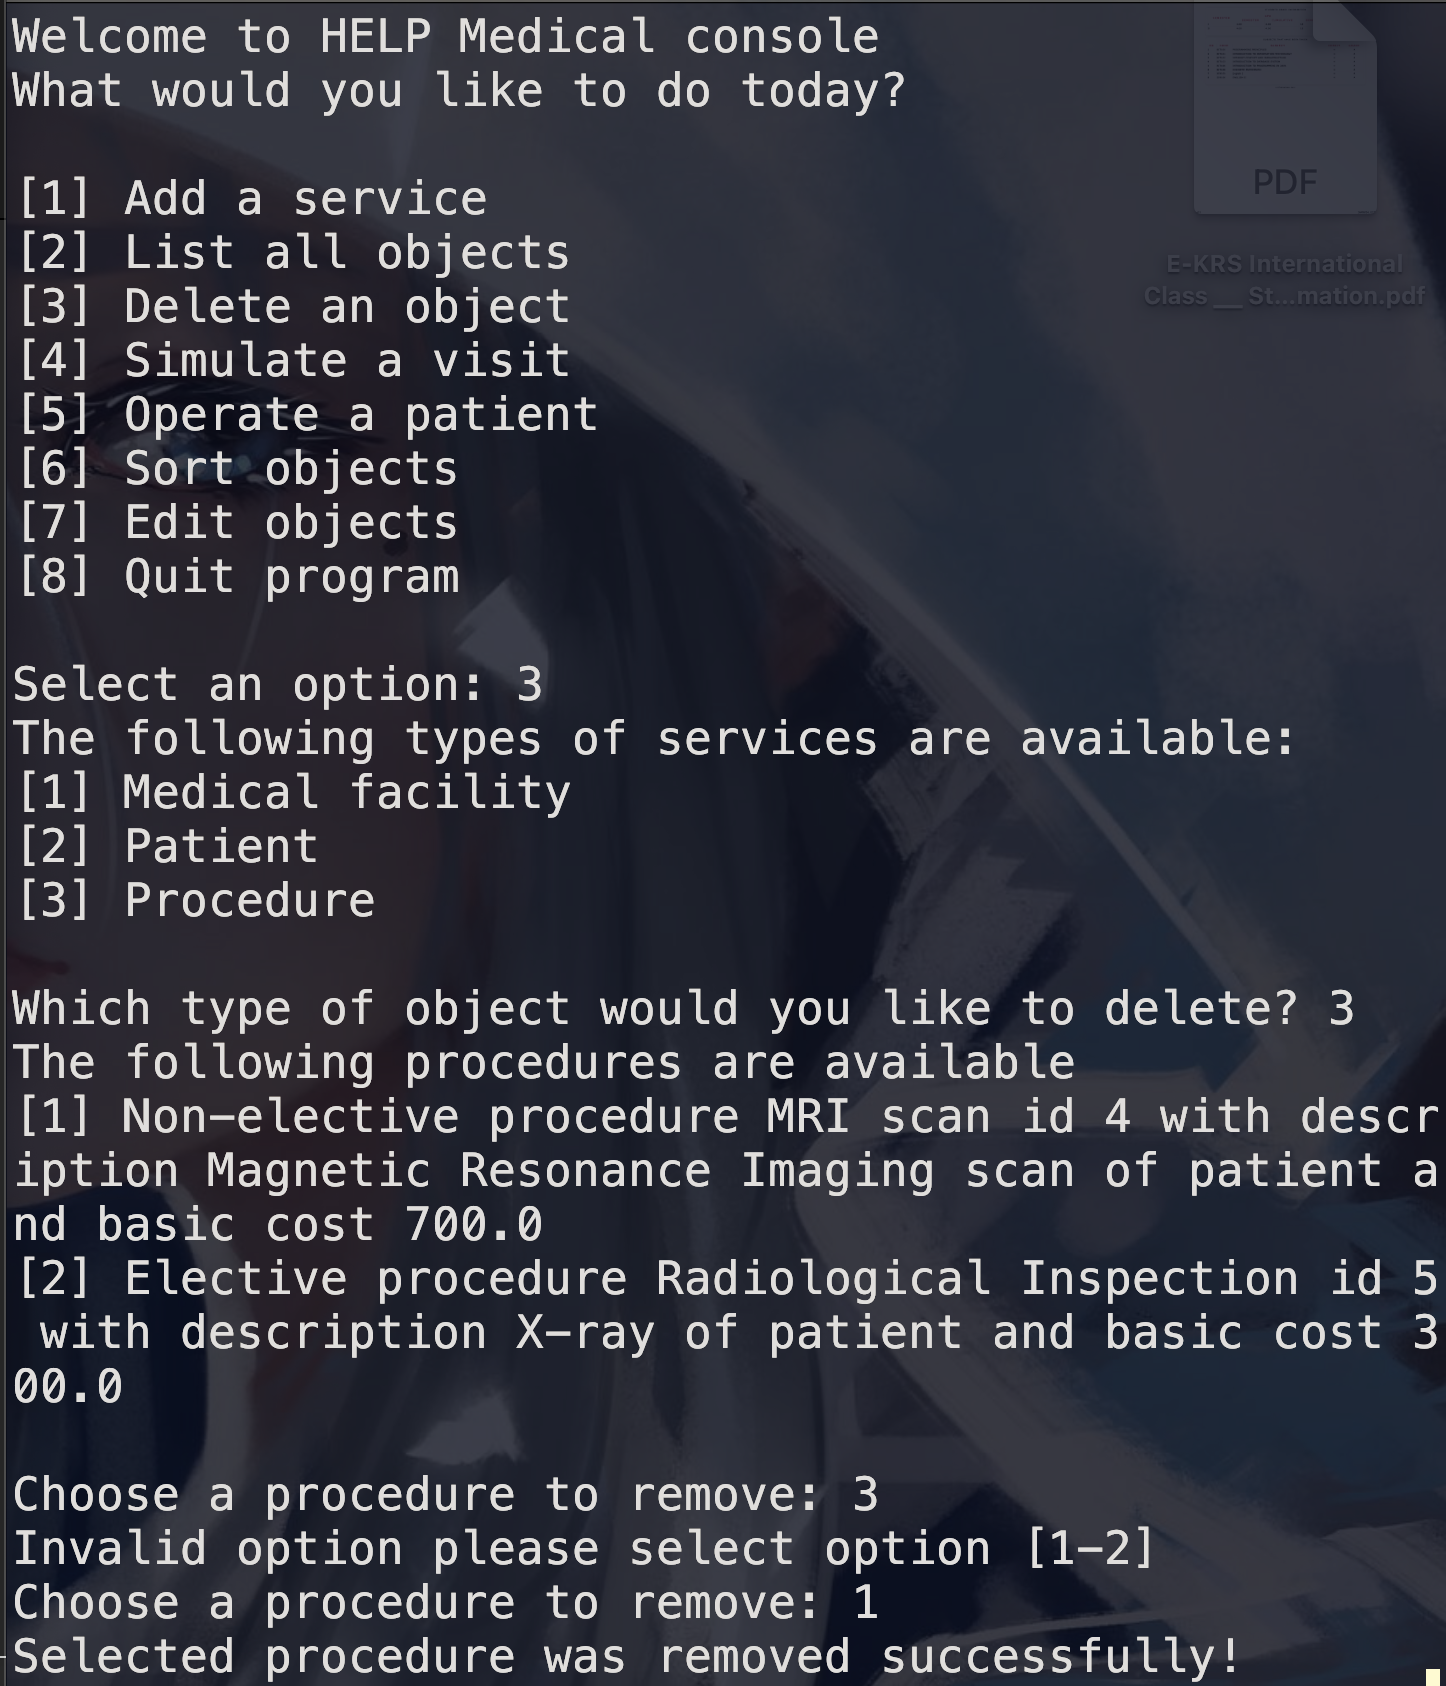
\includegraphics[width=0.6\textwidth]{figures/Deleting/Deleting_Procedure_01.png}
		\end{center}
		\caption{Deleting procedure}\label{fig:deleting_procedure_01}
	\end{figure}
	
	As can be seen, all objects are deleted successfully. To further reinforce this fact, the following list output can be seen:
	\begin{figure}
		\begin{center}
			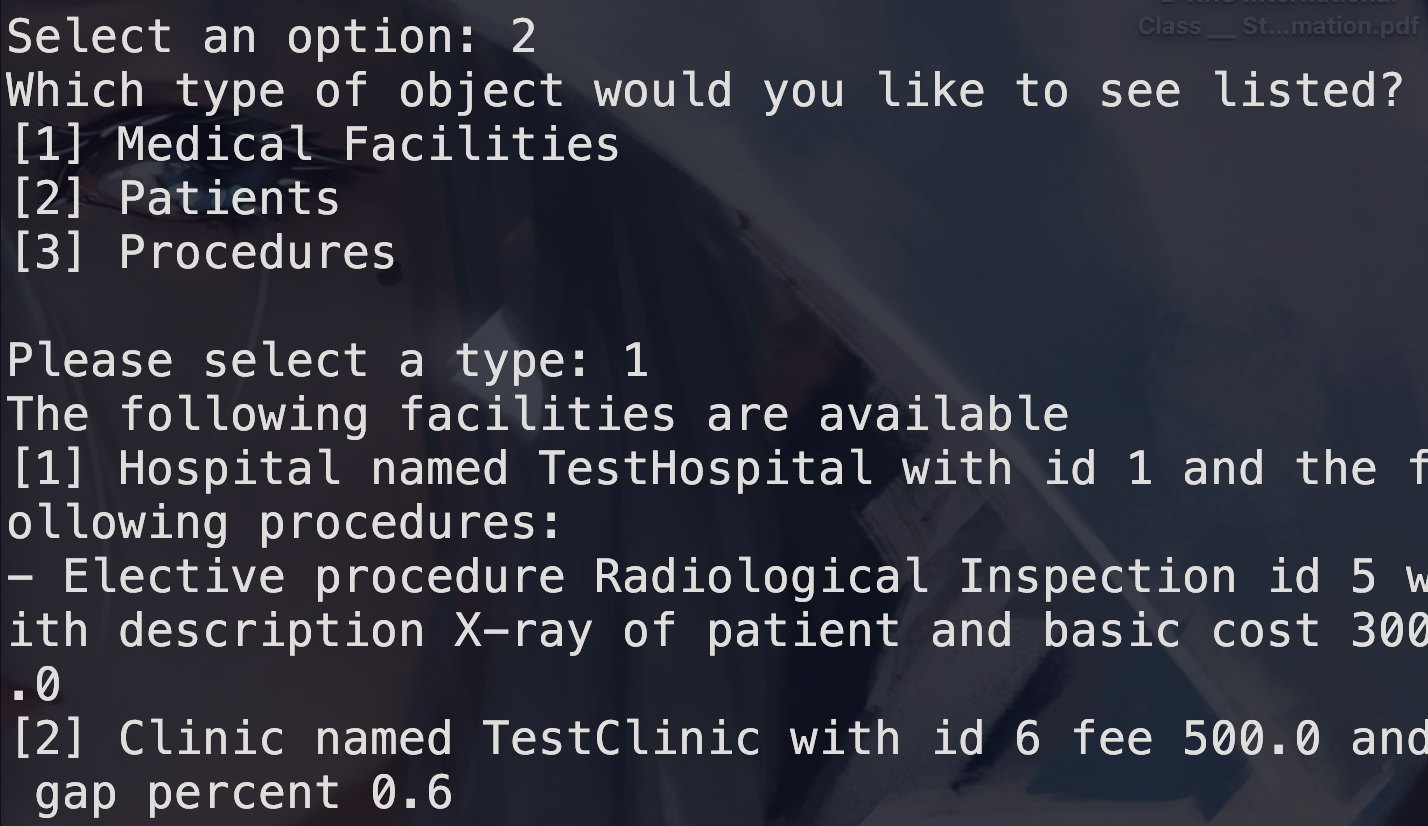
\includegraphics[width=0.6\textwidth]{figures/Deleting/After_deletion_list_01.png}
		\end{center}
		\caption{List output for facilities}\label{fig:after_deletion_01}
	\end{figure}

	\begin{figure}
		\begin{center}
			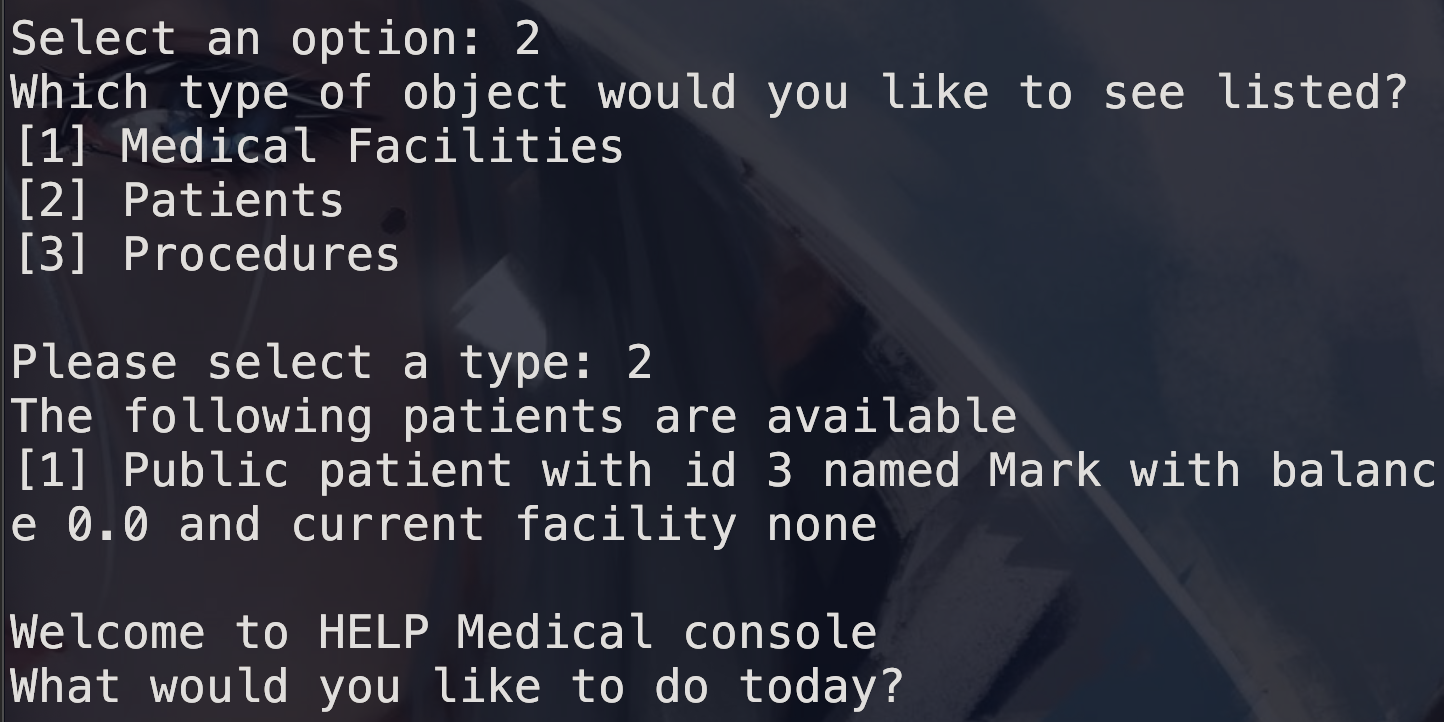
\includegraphics[width=0.6\textwidth]{figures/Deleting/After_deletion_list_02.png}
		\end{center}
		\caption{List output for patients}\label{fig:after_deletion_02}
	\end{figure}

	\begin{figure}
		\begin{center}
			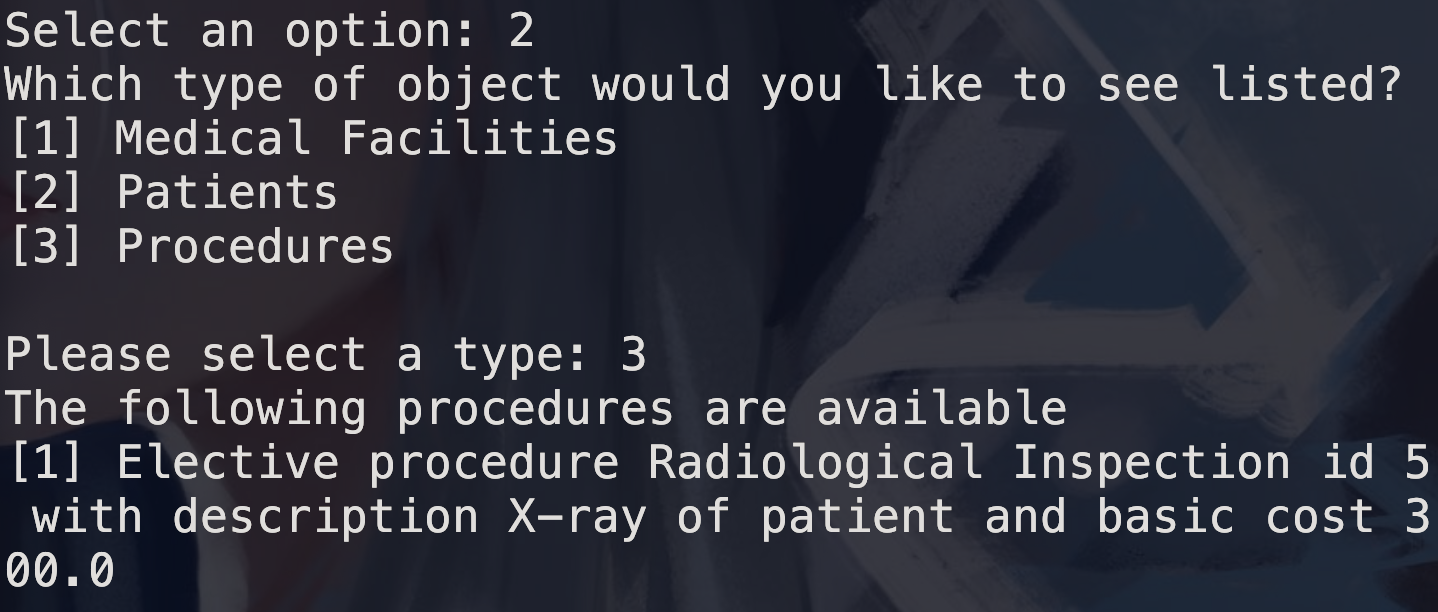
\includegraphics[width=0.6\textwidth]{figures/Deleting/After_deletion_list_03.png}
		\end{center}
		\caption{List output for procedures}\label{fig:after_deletion_03}
	\end{figure}
	% subsection Deleting objects (end)

	\subsection{Simulating a visit}\label{sub:simulating_a_visit} % (fold)
	For these next 2 tests, the base generated data will be used, no other extra data. Tests will also be done separetely.

	\newpage 

	\textit{Registration of patients}
	\begin{figure}
		\begin{center}
			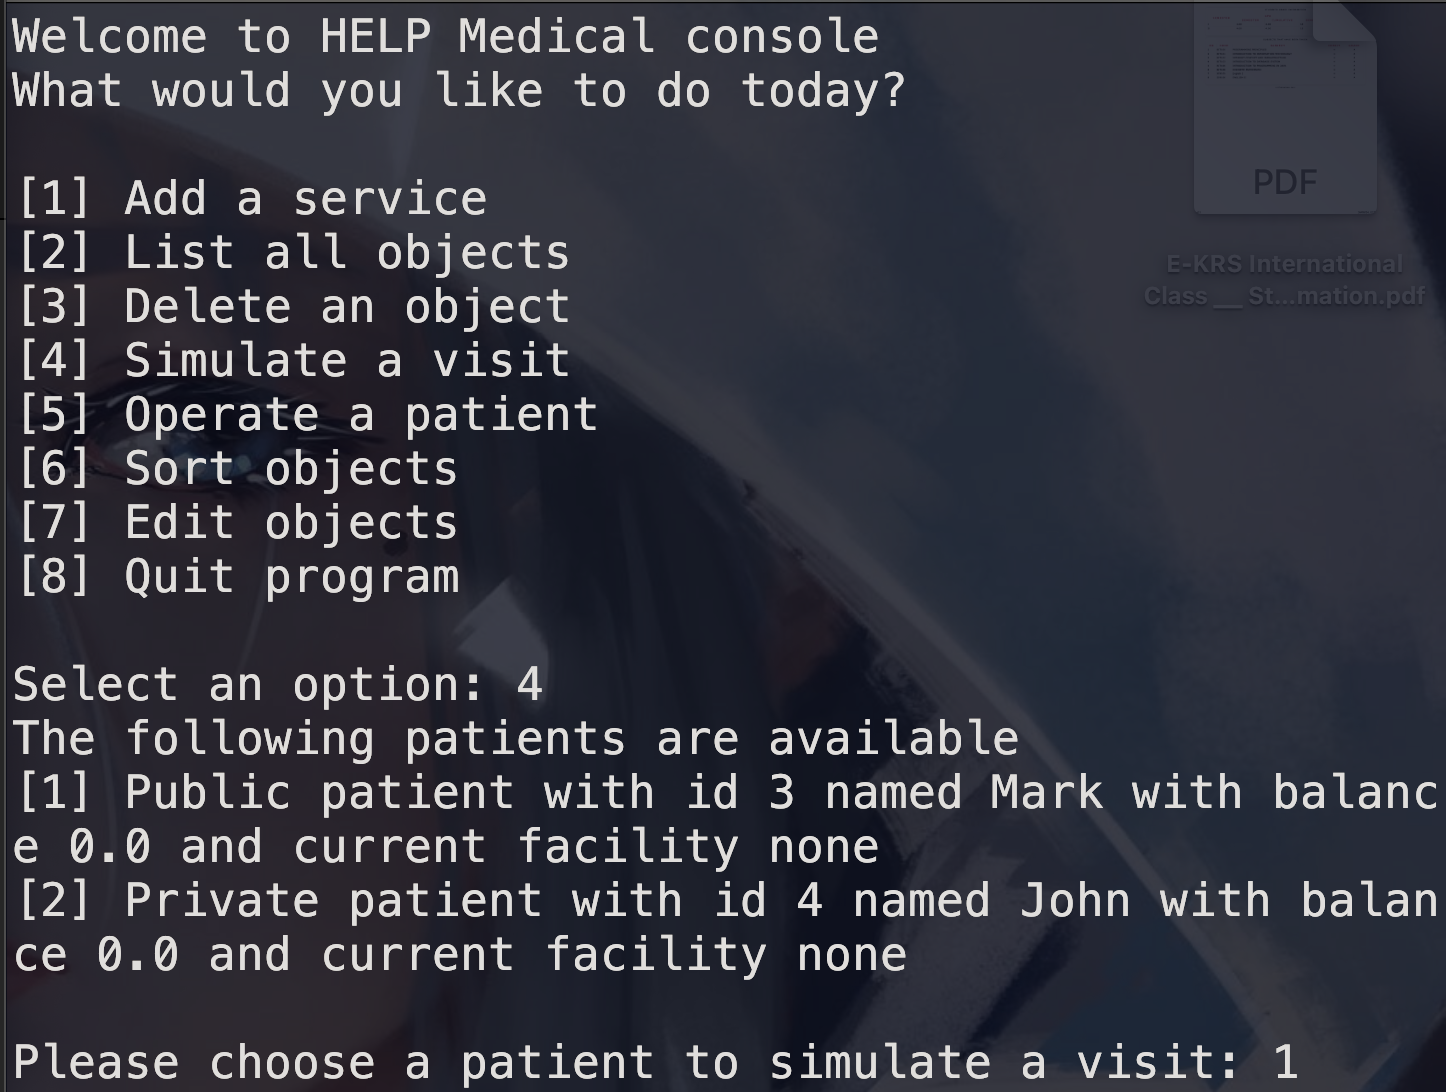
\includegraphics[width=0.6\textwidth]{figures/Visiting/Register_patients_01.png}
		\end{center}
		\caption{Getting to registration pane}\label{fig:register_patients_01}
	\end{figure}

	\begin{figure}
		\begin{center}
			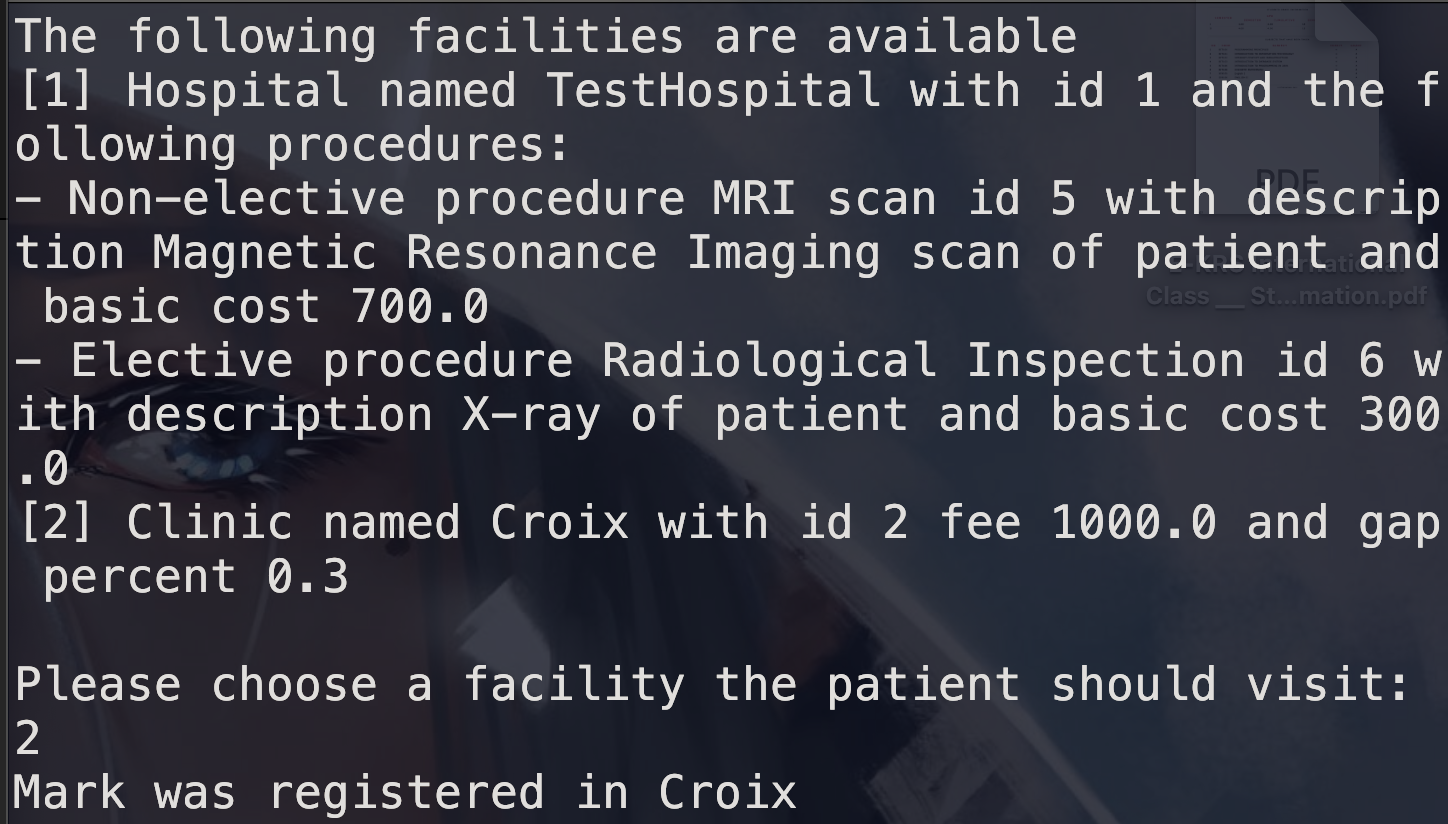
\includegraphics[width=0.6\textwidth]{figures/Visiting/Register_patients_02.png}
		\end{center}
		\caption{Registering patient 1}\label{fig:register_patients_02}
	\end{figure}
	
	\begin{figure}
		\begin{center}
			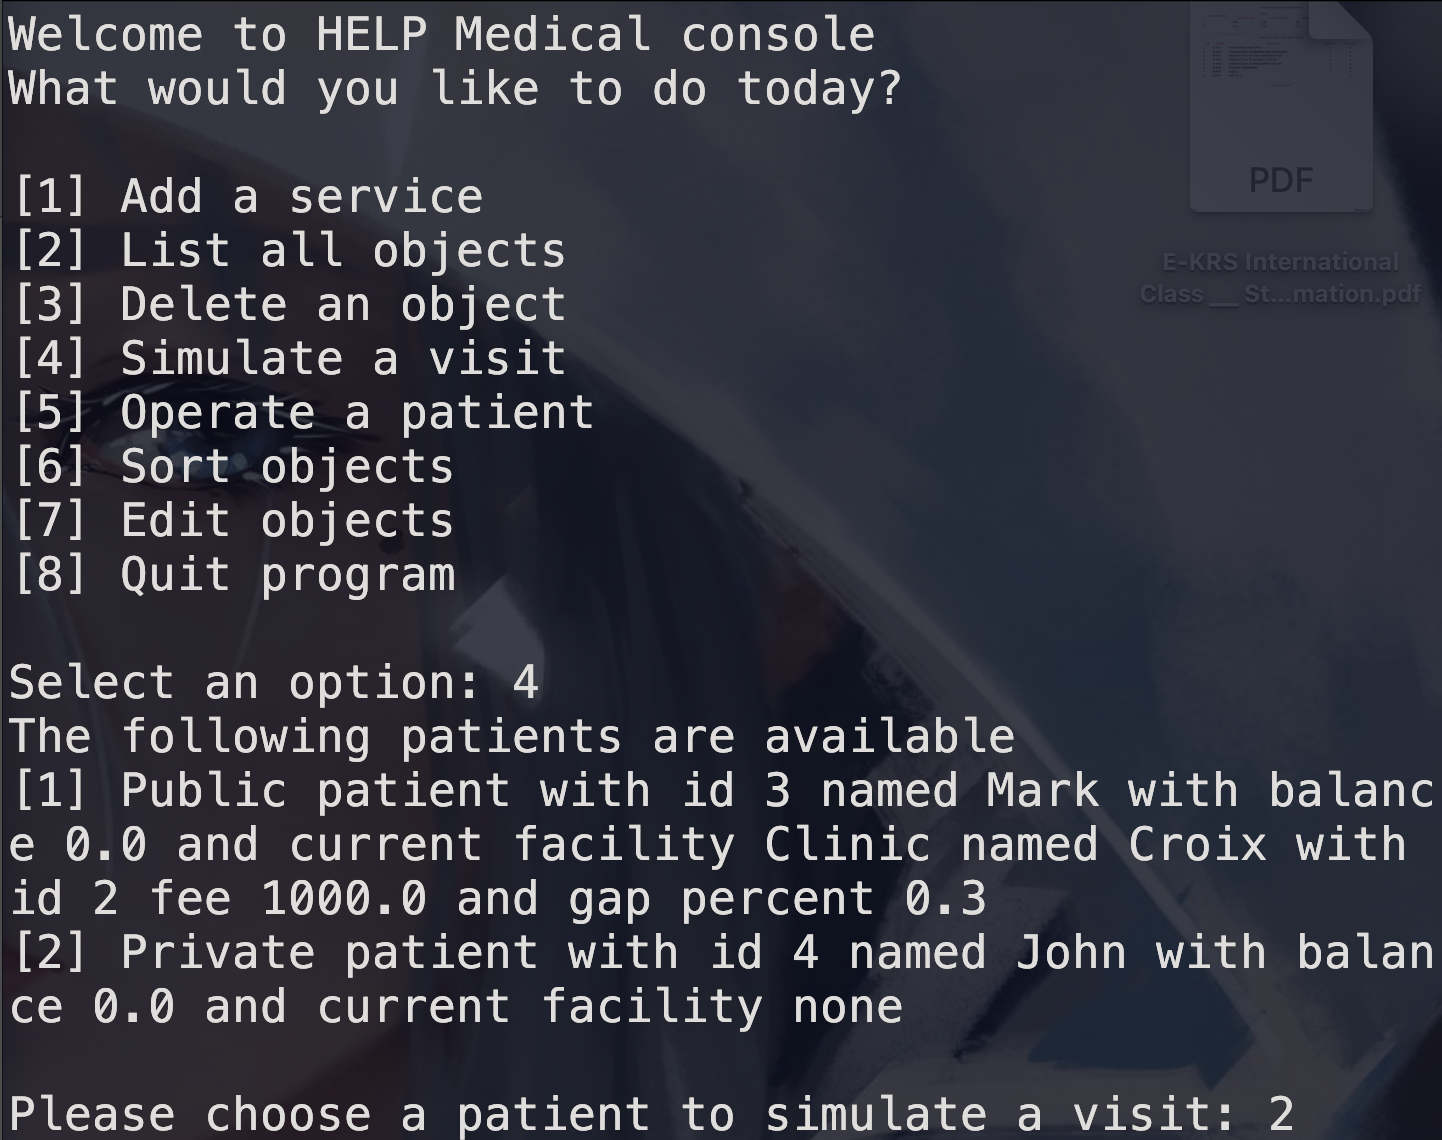
\includegraphics[width=0.6\textwidth]{figures/Visiting/Register_patients_03.png}
		\end{center}
		\caption{Getting to registration pane}\label{fig:register_patients_03}
	\end{figure}

	\begin{figure}
		\begin{center}
			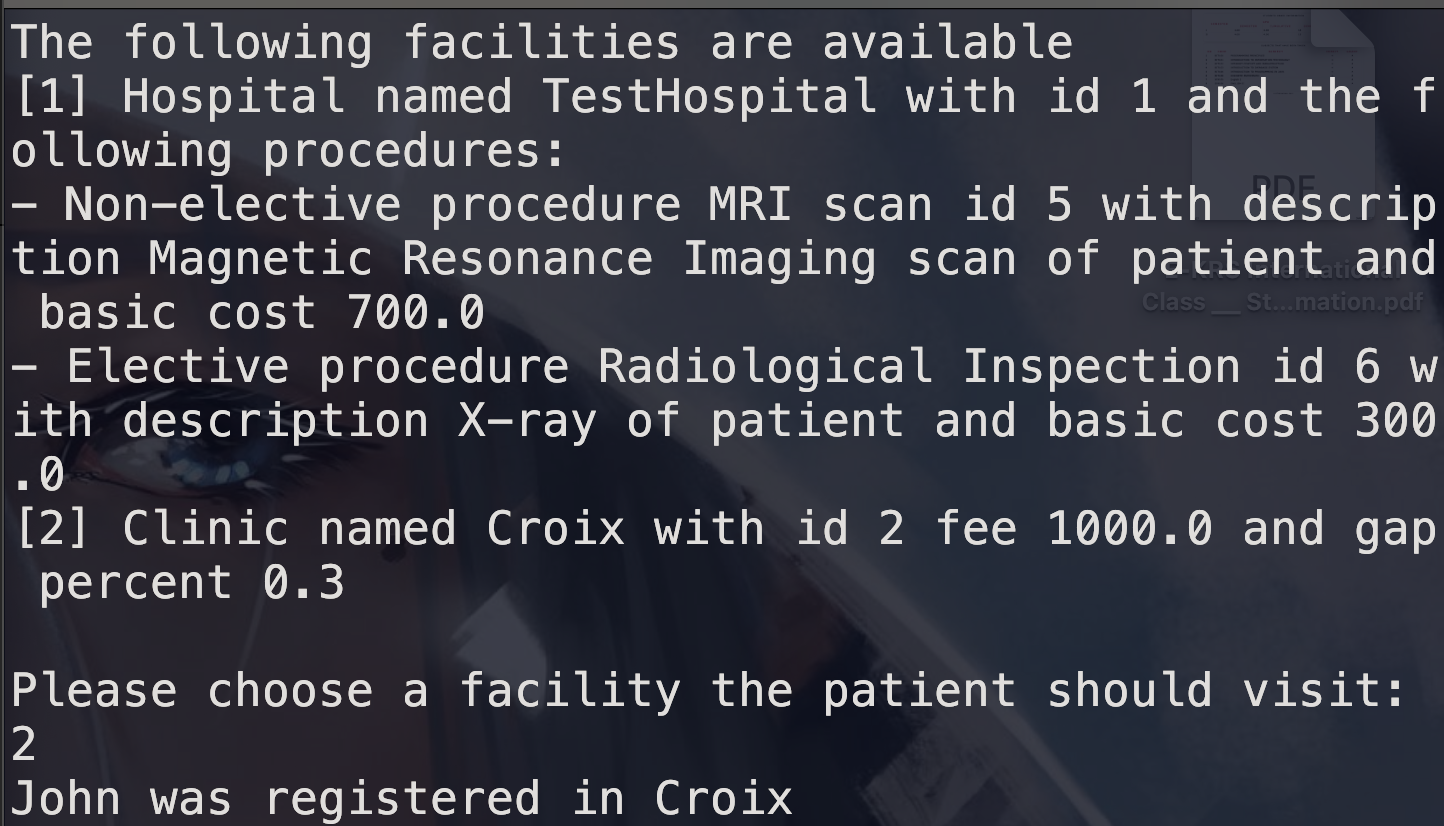
\includegraphics[width=0.6\textwidth]{figures/Visiting/Register_patients_04.png}
		\end{center}
		\caption{Registering patient 1}\label{fig:register_patients_04}
	\end{figure}


	\newpage 


	\textit{Subsequent visits by patients}
	\begin{figure}
		\begin{center}
			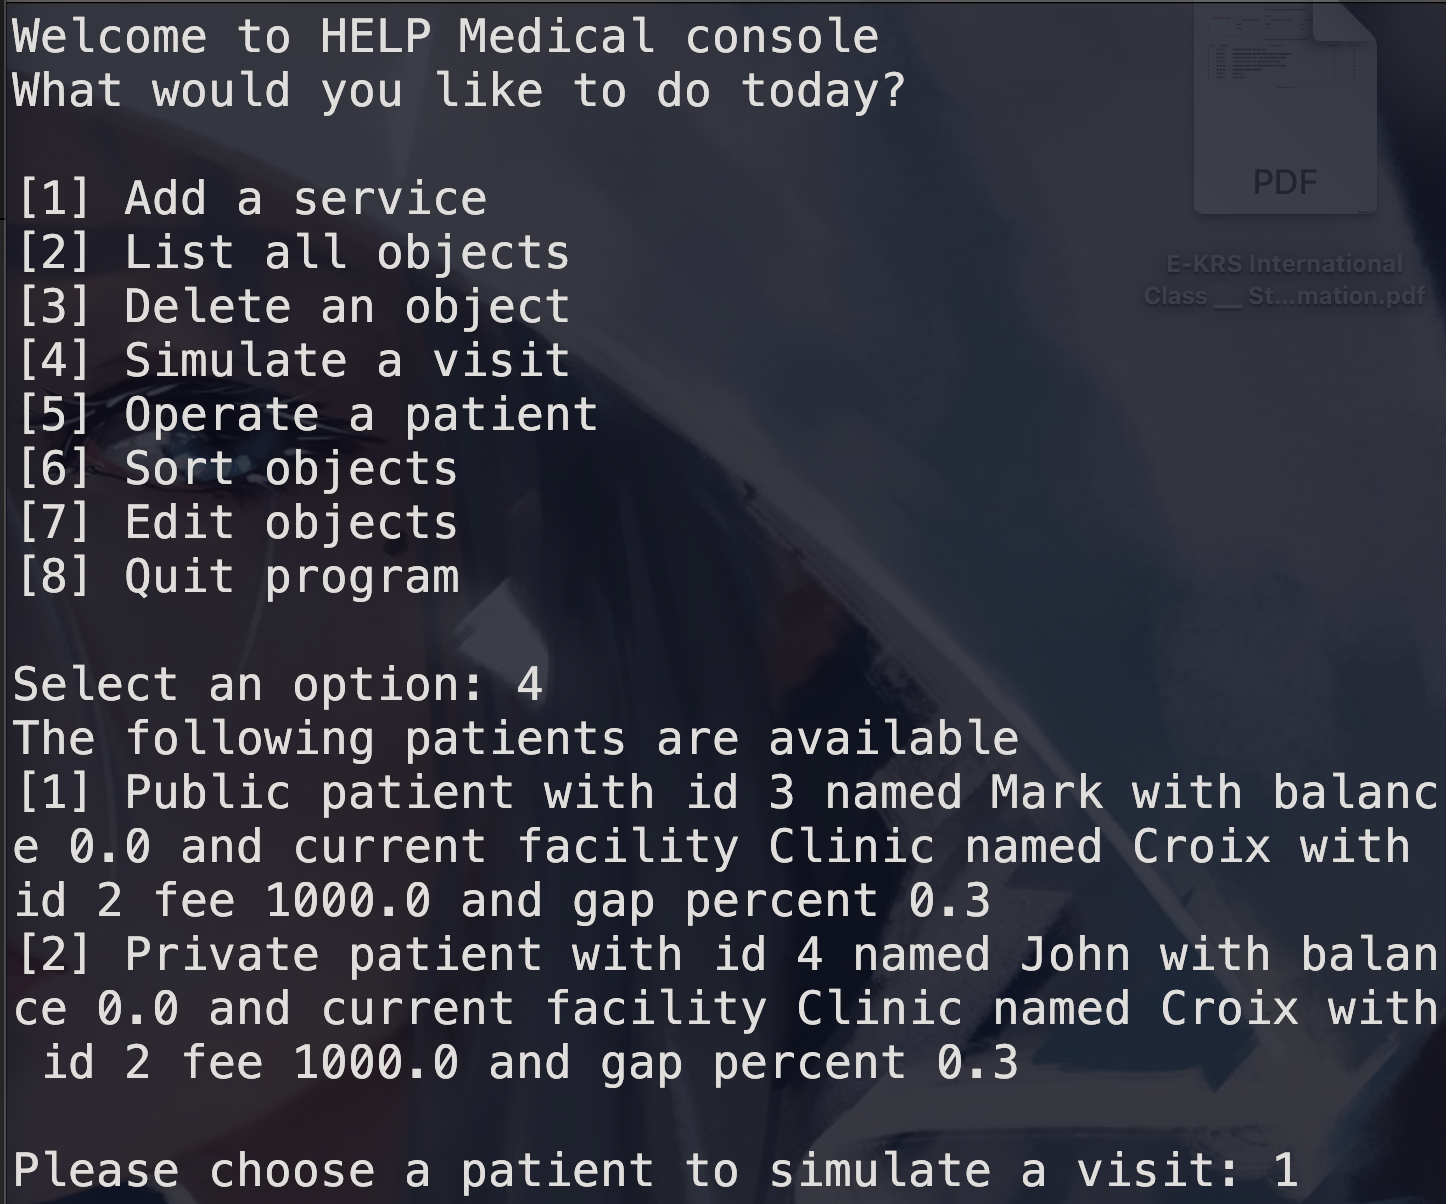
\includegraphics[width=0.6\textwidth]{figures/Visiting/Visit_with_patients_01.png}
		\end{center}
		\caption{Getting to the visit pane}\label{fig:visit_with_patients_01}
	\end{figure}

	\begin{figure}
		\begin{center}
			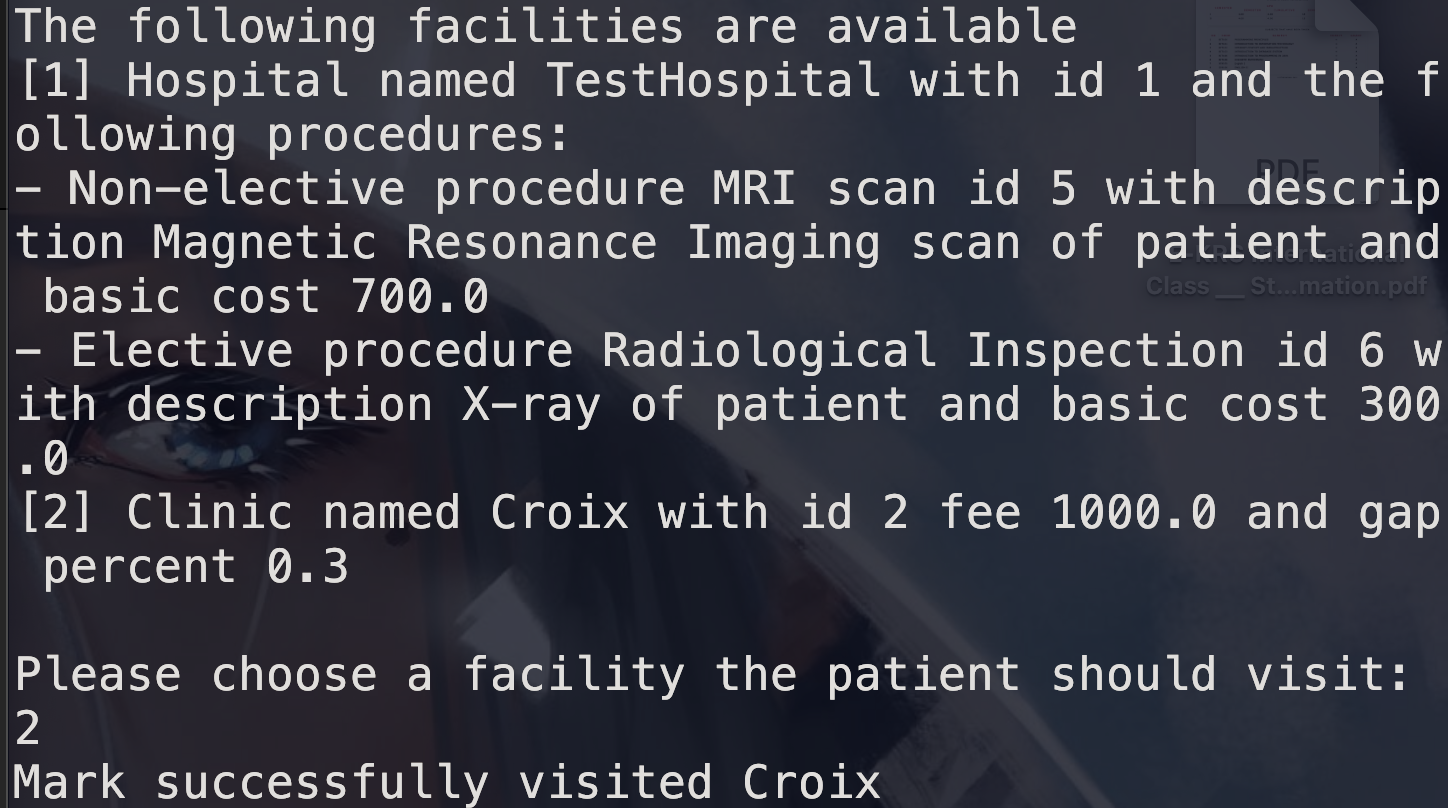
\includegraphics[width=0.6\textwidth]{figures/Visiting/Visit_with_patients_02.png}
		\end{center}
		\caption{Visiting with patient 1}\label{fig:visit_with_patients_02}
	\end{figure}

	\begin{figure}
		\begin{center}
			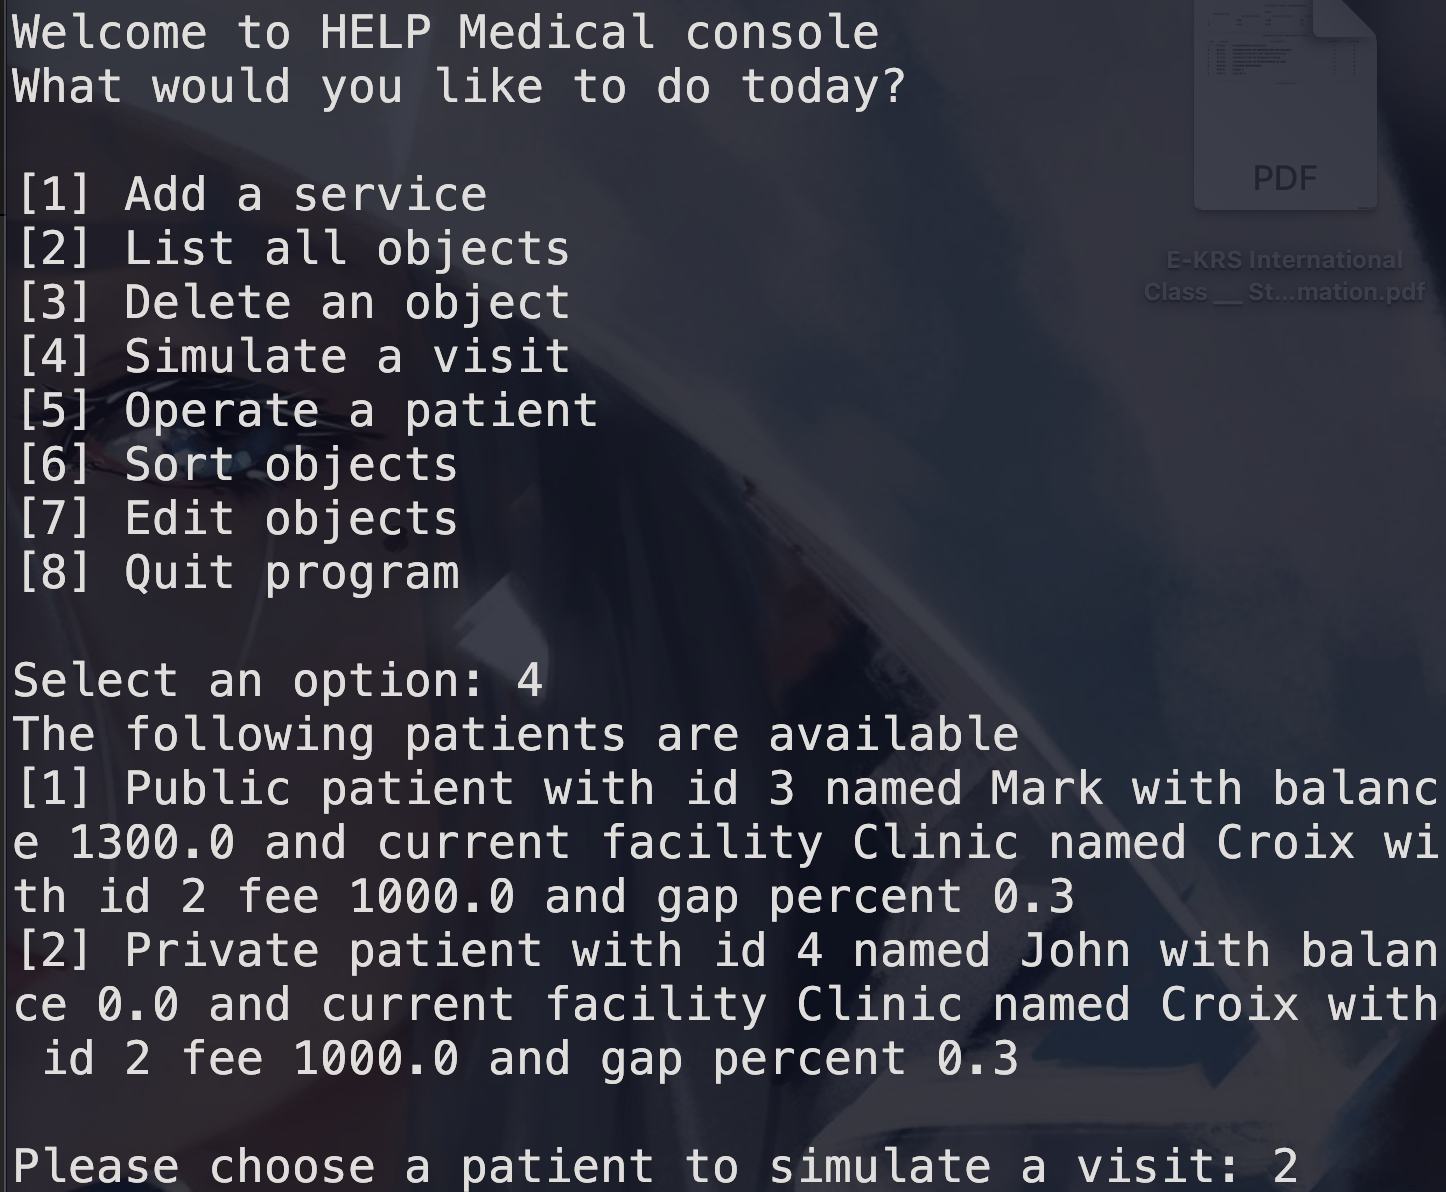
\includegraphics[width=0.6\textwidth]{figures/Visiting/Visit_with_patients_03.png}
		\end{center}
		\caption{Getting to the visit pane}\label{fig:visit_with_patients_03}
	\end{figure}

	\begin{figure}
		\begin{center}
			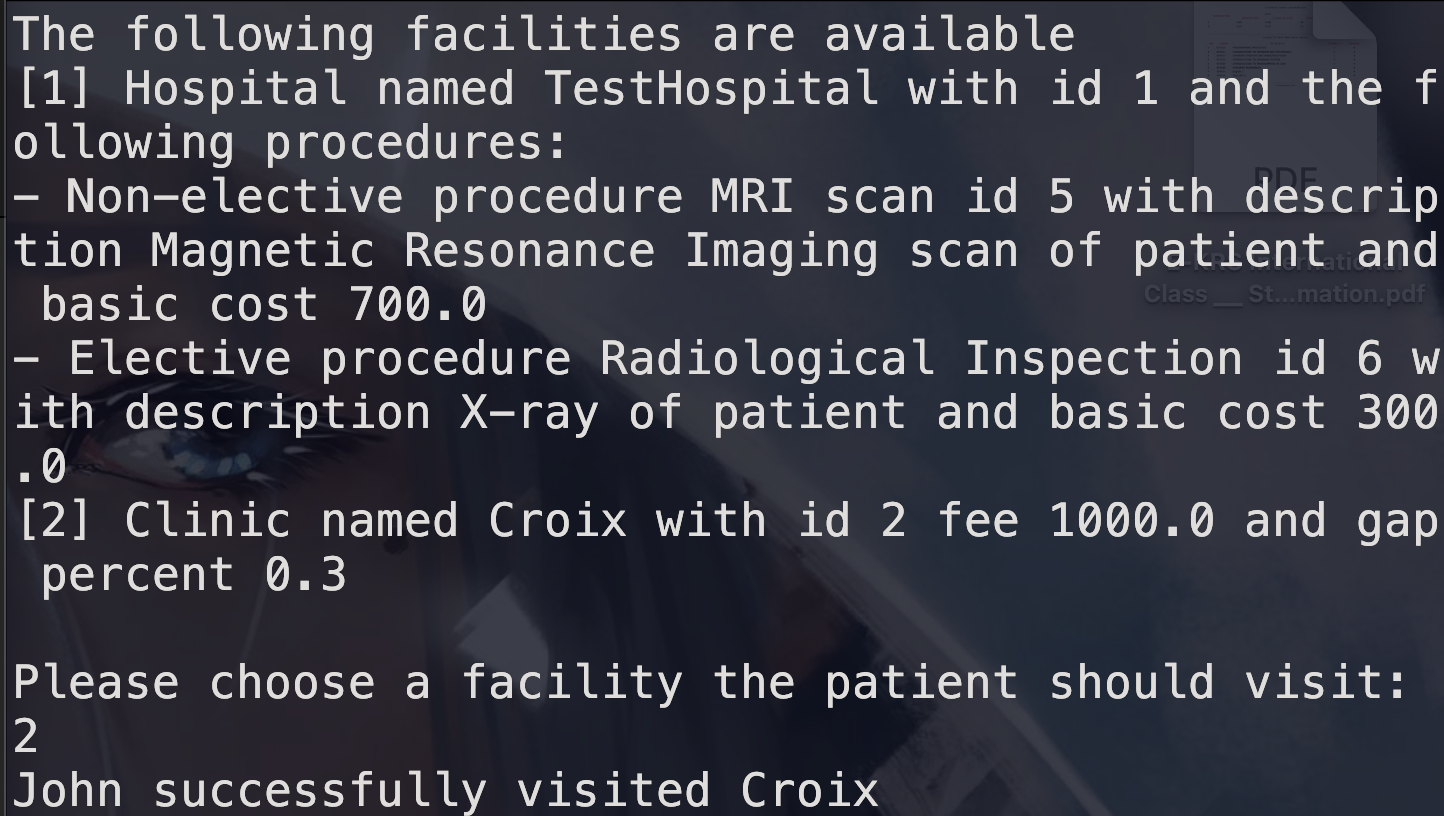
\includegraphics[width=0.6\textwidth]{figures/Visiting/Visit_with_patients_04.png}
		\end{center}
		\caption{Visiting with patient 2}\label{fig:visit_with_patients_04}
	\end{figure}

	\begin{figure}
		\begin{center}
			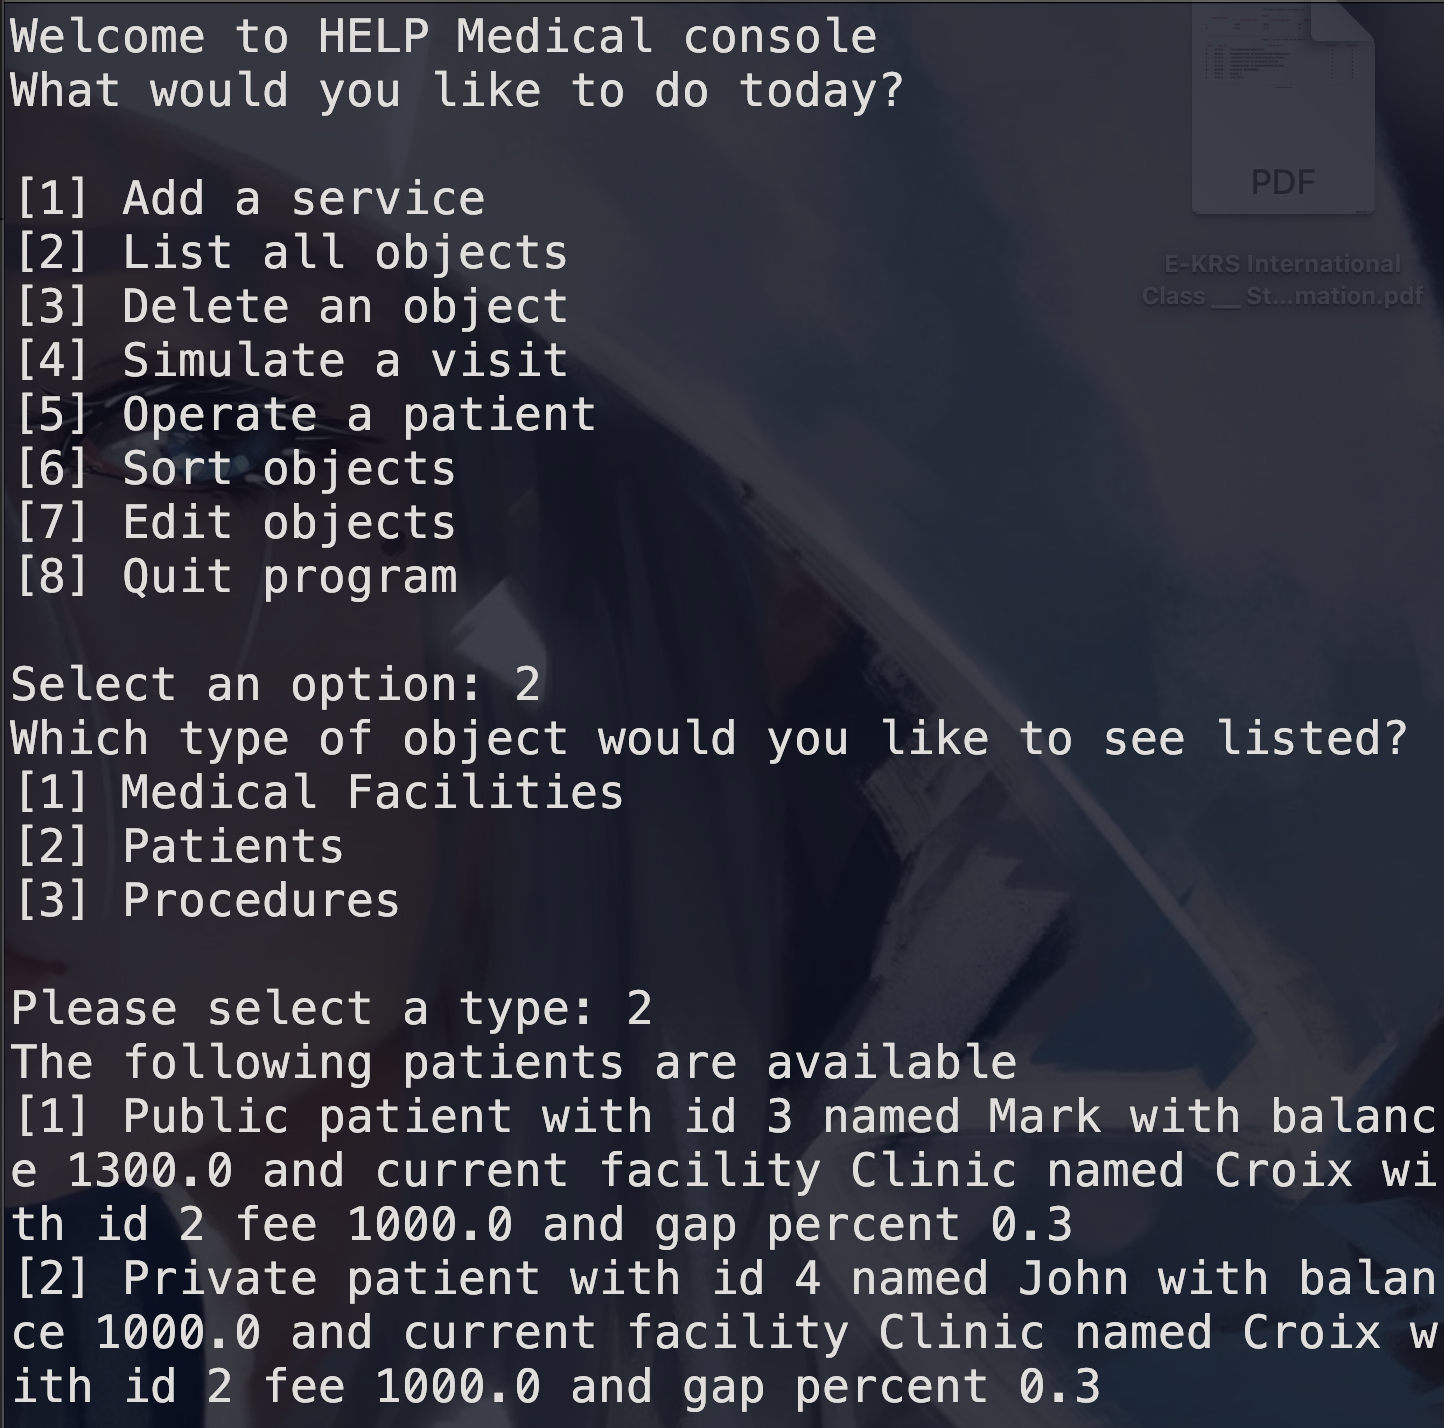
\includegraphics[width=0.6\textwidth]{figures/Visiting/Result_patient_visit.png}
		\end{center}
		\caption{Results of patient visit}\label{fig:result_patient_visit}
	\end{figure}

	As can be seen, the added balances are correct for both patients. This is because for the private patient, the cost is equal to the fee attribute of the clinic, meanwhile for the public patient, using the formula below: 
	\[
		1000.0 + (1000 * 0.3)
	\]
	\[
		1000.0 + 300 = 1300.0
	\]


	\newpage 

	\textit{Visit hospital}
	\begin{figure}
		\begin{center}
			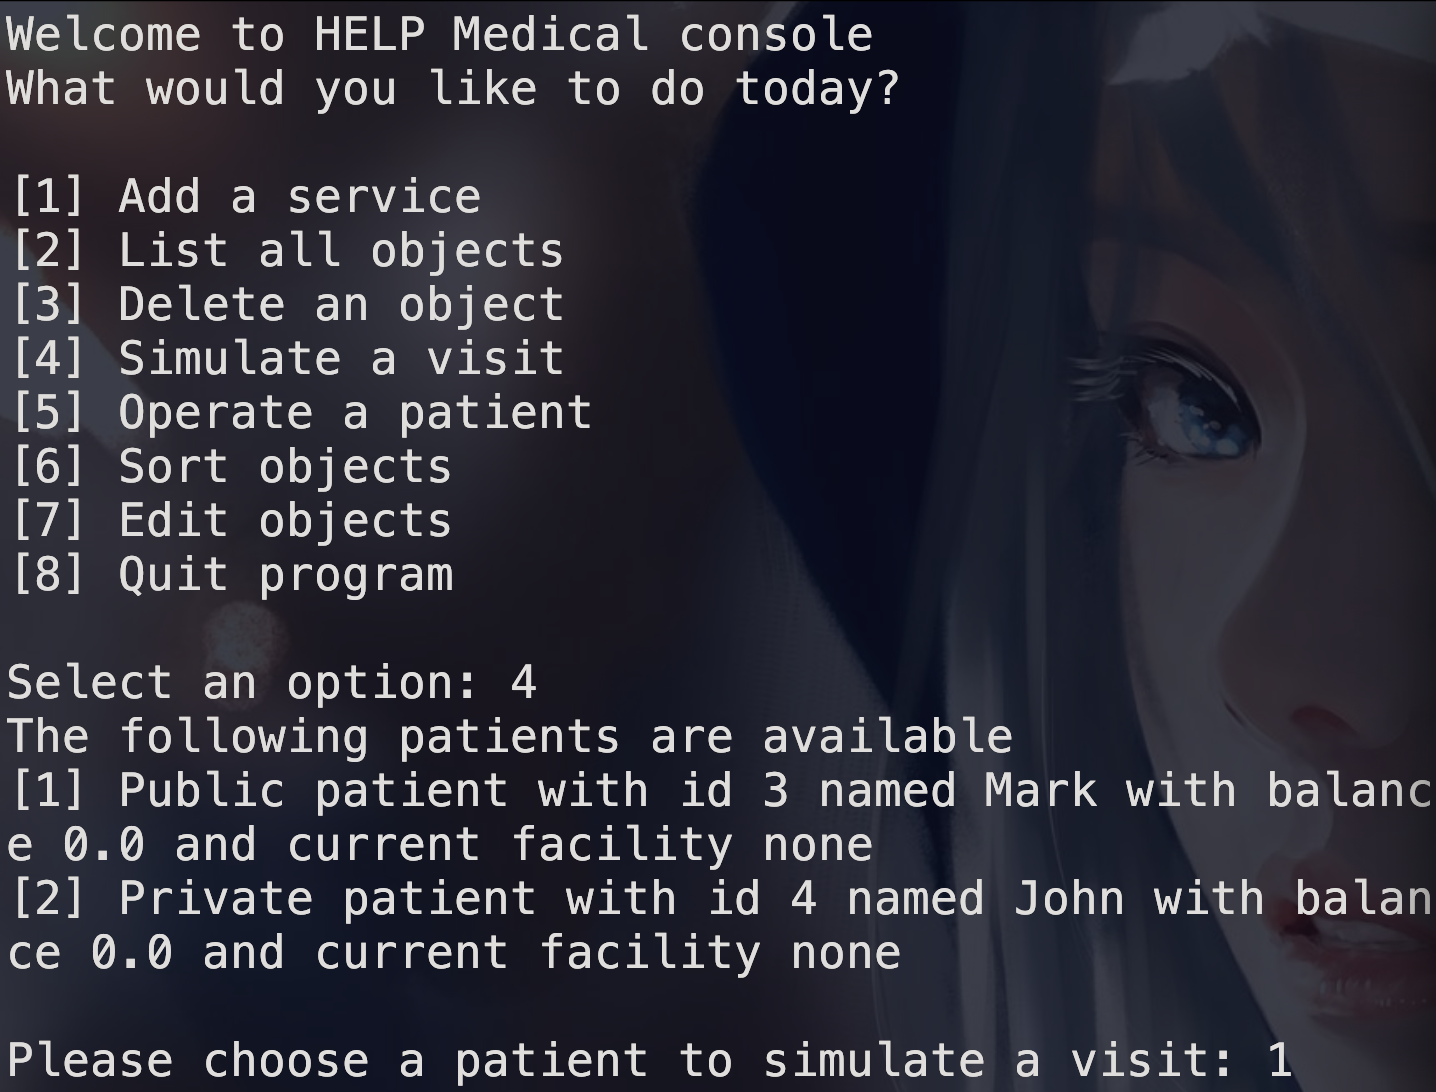
\includegraphics[width=0.6\textwidth]{figures/Visiting/Register_hospital_01.png}
		\end{center}
		\caption{Getting to the registration pane}\label{fig:register_hospital_01}
	\end{figure}

	\begin{figure}
		\begin{center}
			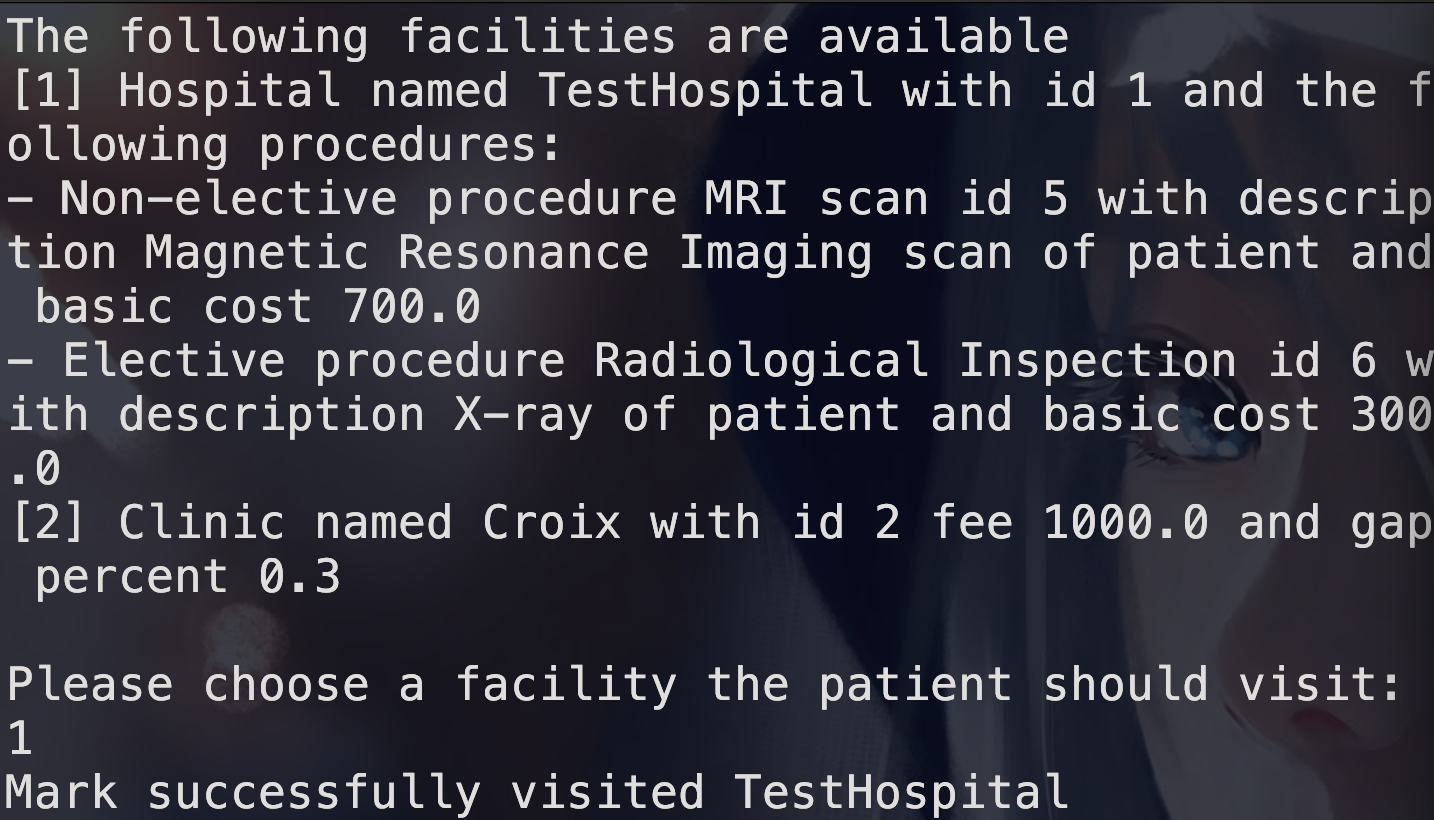
\includegraphics[width=0.6\textwidth]{figures/Visiting/Register_hospital_02.png}
		\end{center}
		\caption{Registering patient to hospital}\label{fig:register_hospital_02}
	\end{figure}
	
	% subsection Simulating a visit (end)

	\newpage

	\subsection{Simulating an operation}\label{sub:simulating_an_operation} % (fold)
	Due to the fact that patients can be discharged any time at random after an operation has been undertaken, this runtime test is only undertaken once using a patient that is already registered to the hospital. If one wishes to see a full test which includes all operation possibilities, please check the \ref{sec:unit_tests}
	\begin{figure}
		\begin{center}
			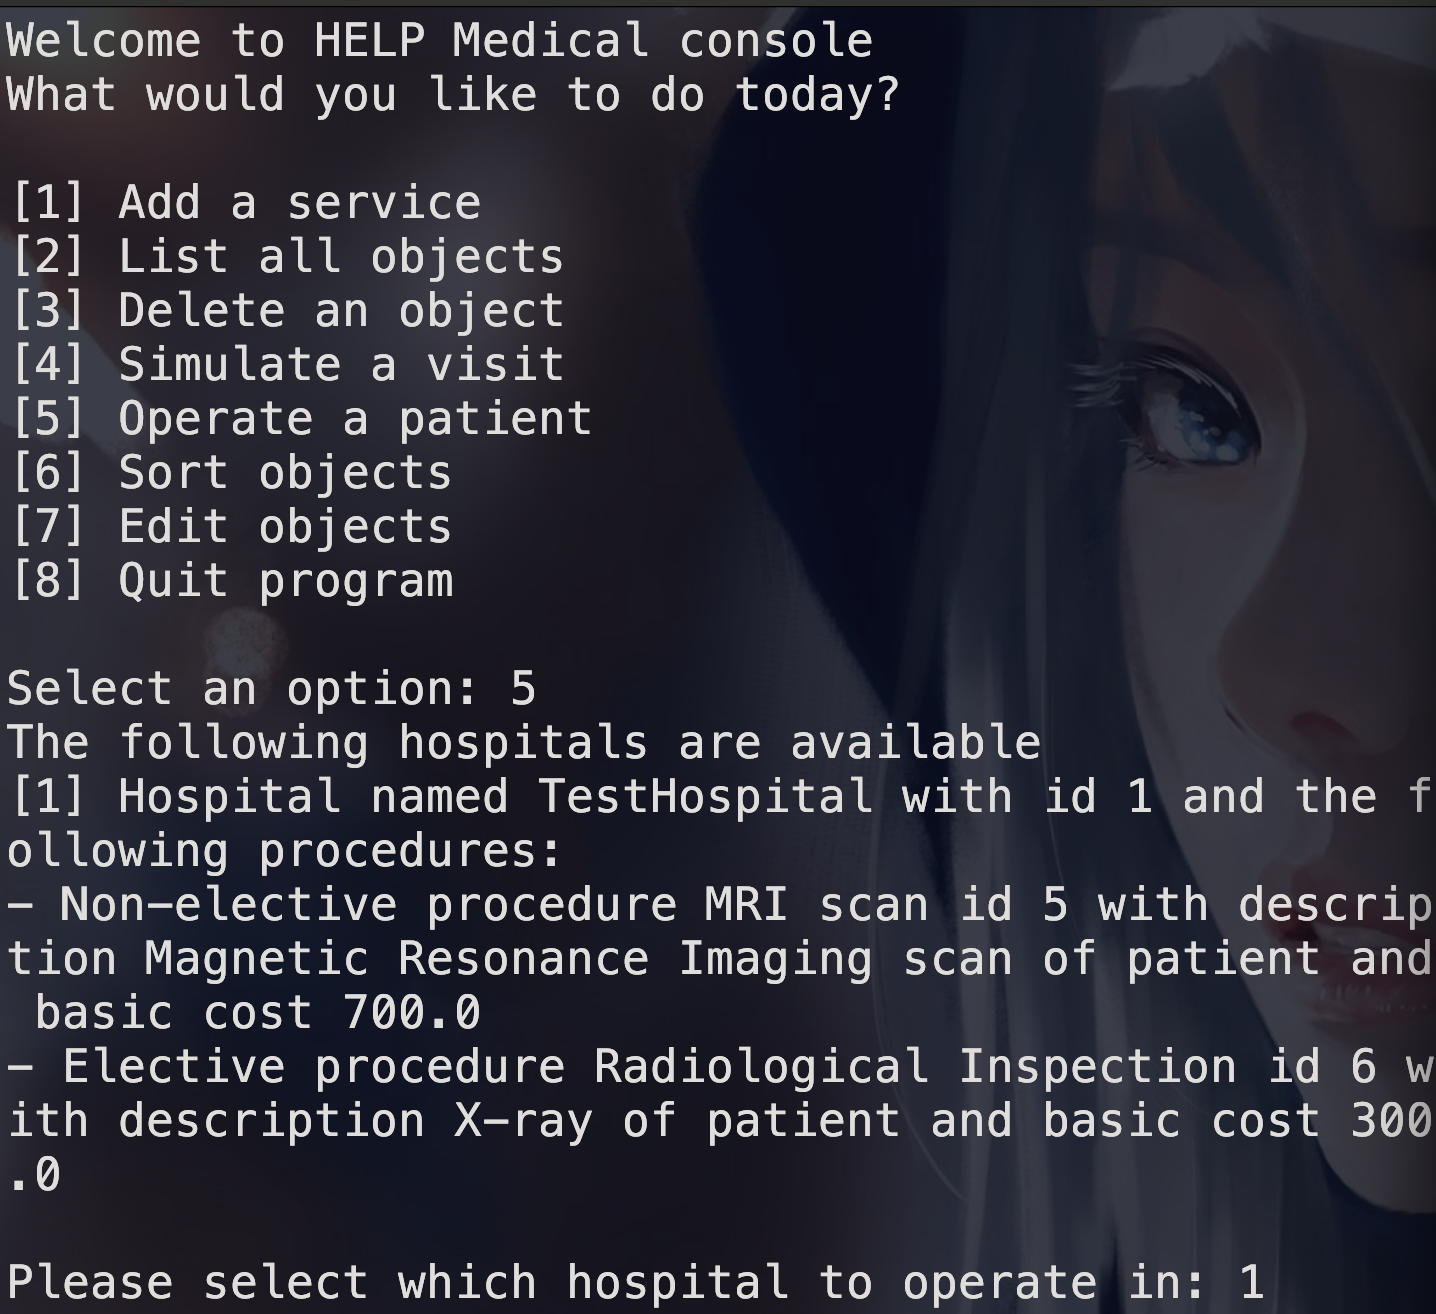
\includegraphics[width=0.6\textwidth]{figures/Operating/Operating_hospital_01.png}
		\end{center}
		\caption{Getting to the operating pane}\label{fig:operating_hospital_01}
	\end{figure}

	\begin{figure}
		\begin{center}
			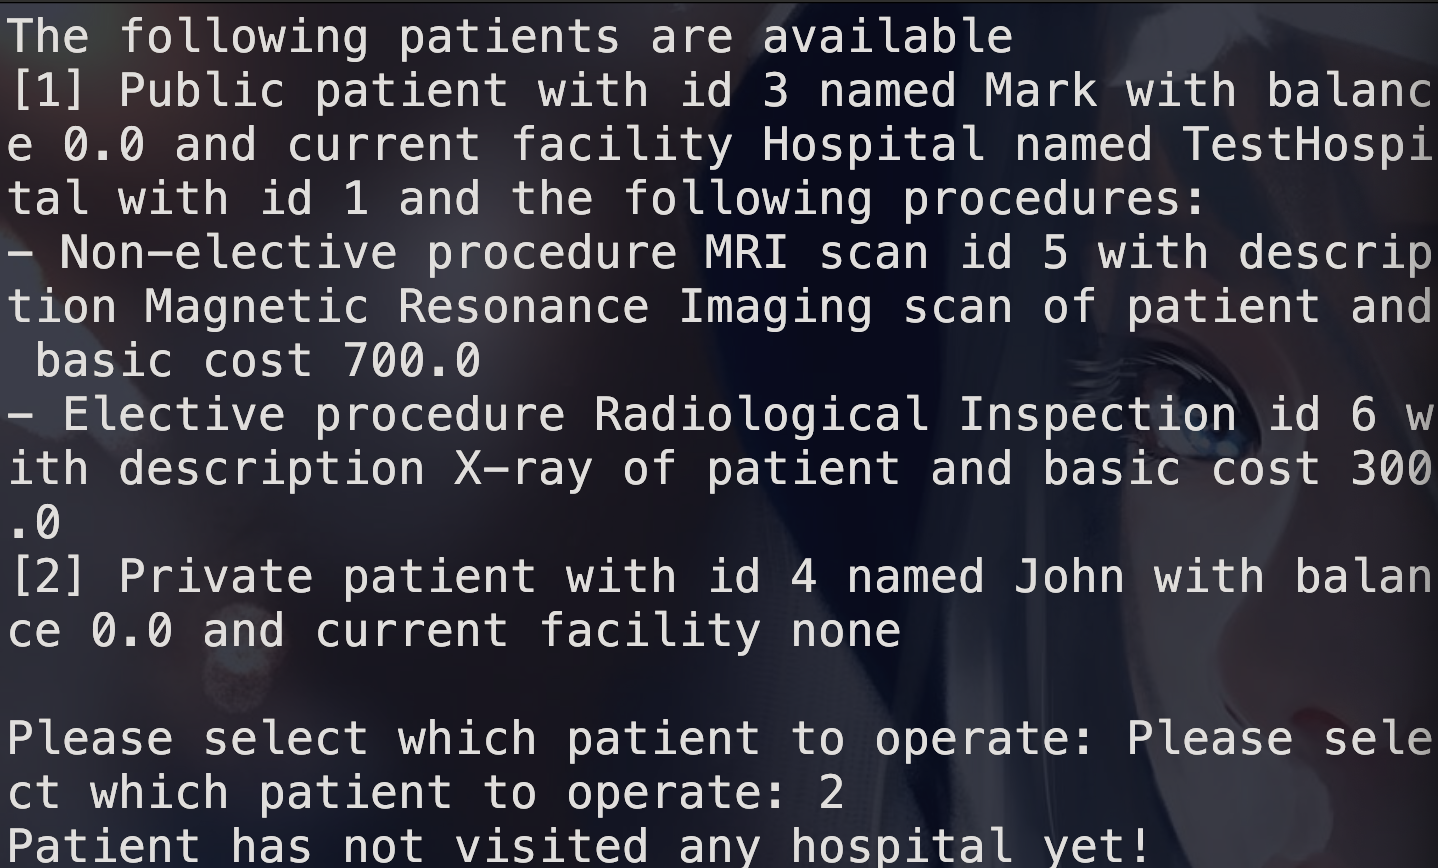
\includegraphics[width=0.6\textwidth]{figures/Operating/Operating_hospital_02.png}
		\end{center}
		\caption{Output when patient is not in the hospital}\label{fig:operating_hospital_02}
	\end{figure}

	\begin{figure}
		\begin{center}
			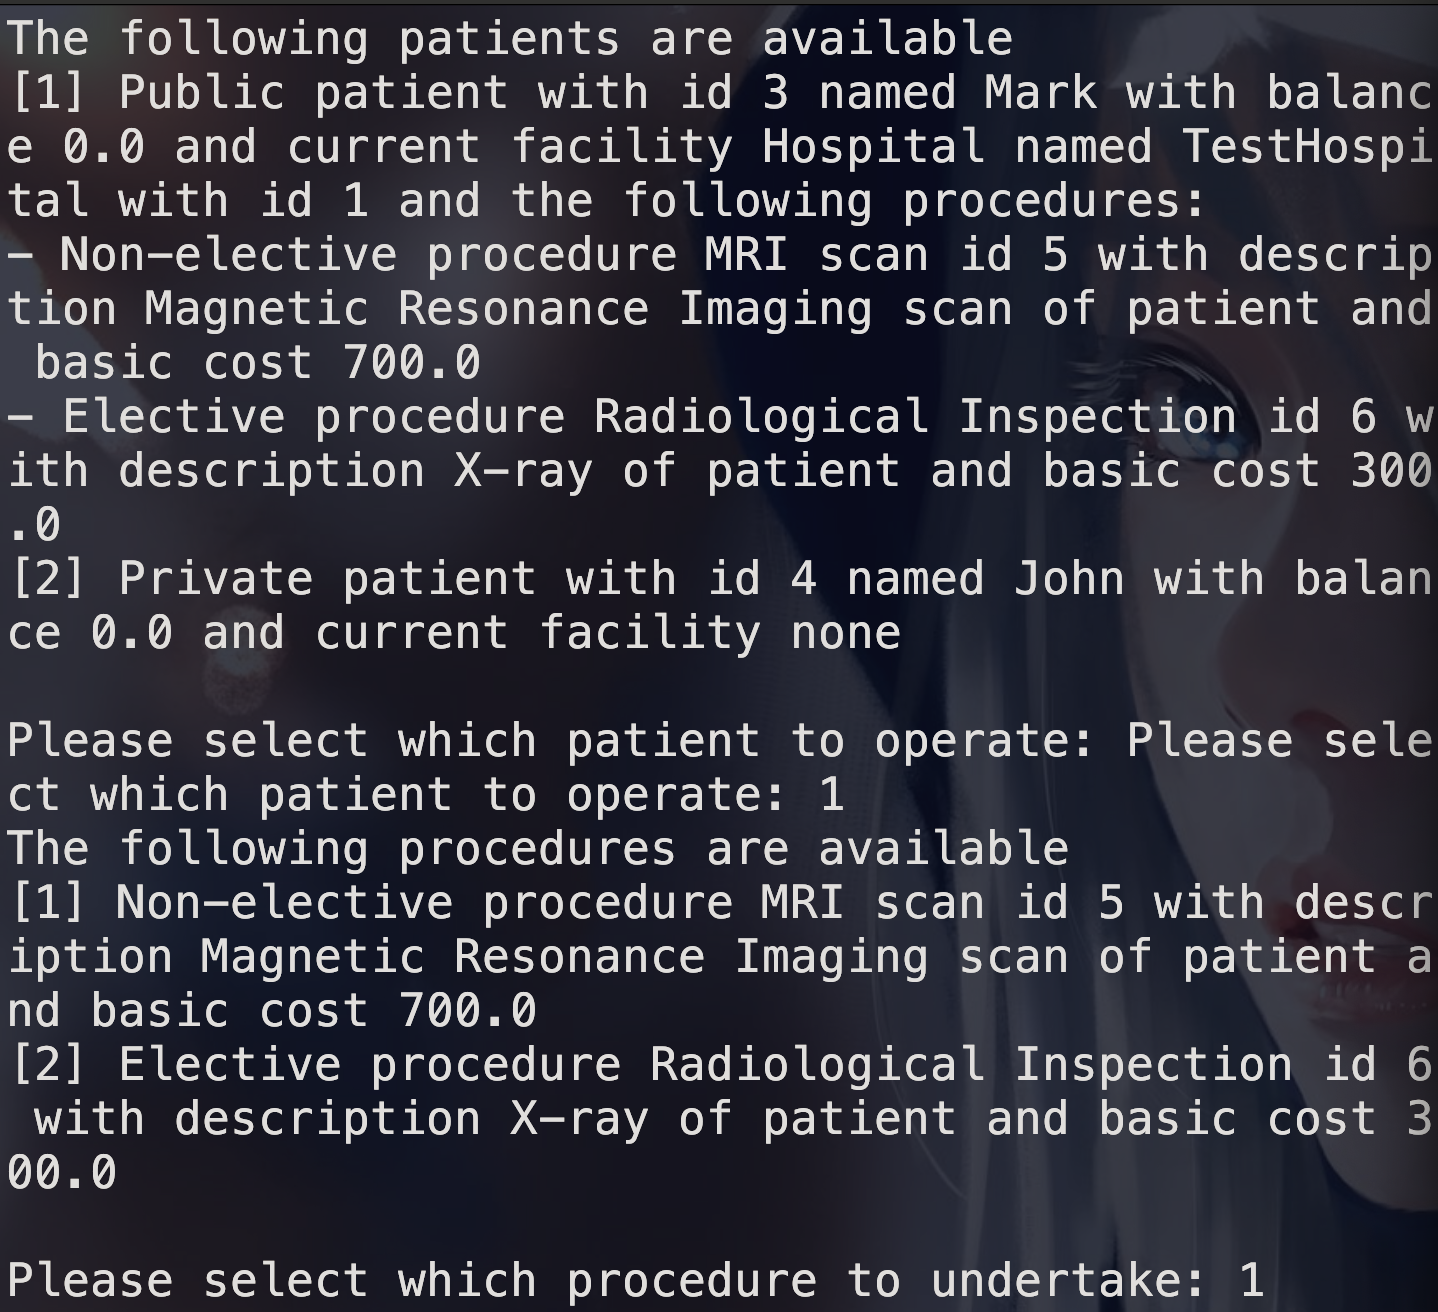
\includegraphics[width=0.6\textwidth]{figures/Operating/Operating_hospital_03.png}
		\end{center}
		\caption{Output when patient is not in the hospital}\label{fig:operating_hospital_03}
	\end{figure}

	When a patient is in the wrong hospital, "Patient is not in this hospital!" is output instead.

	\textit{Results}
	\begin{figure}
		\begin{center}
			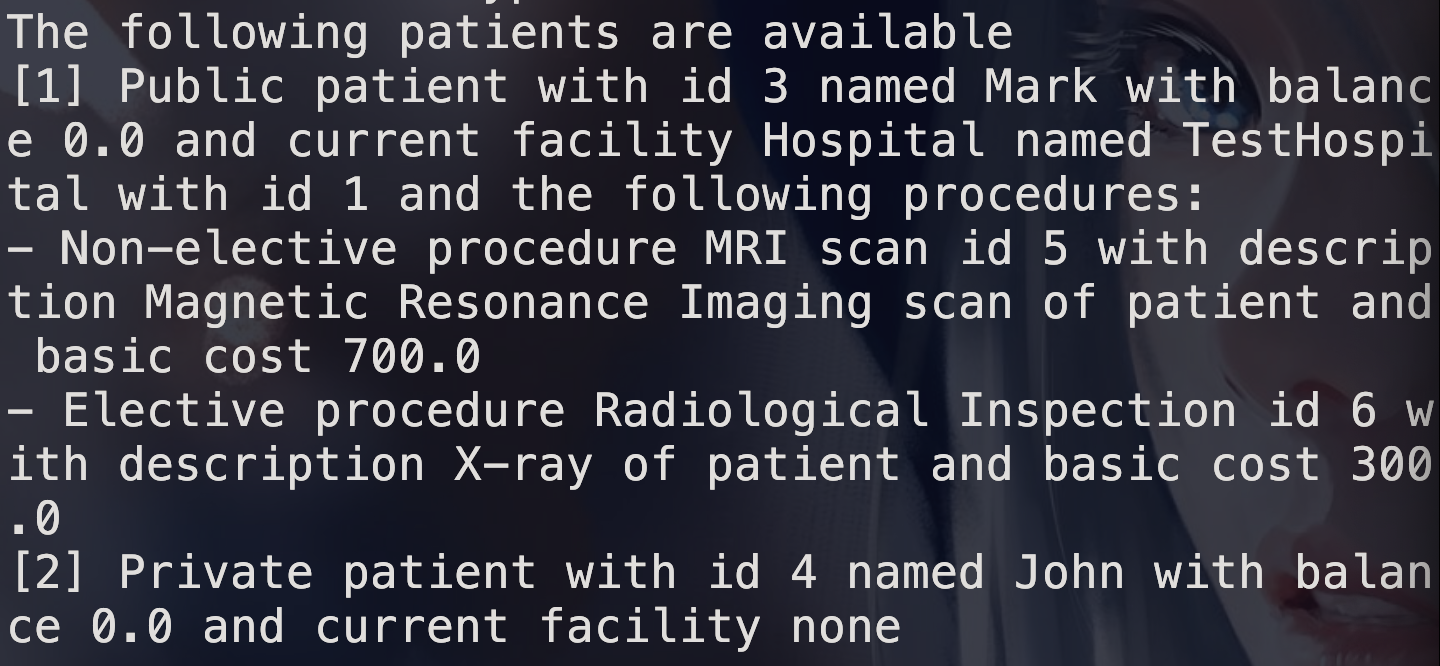
\includegraphics[width=0.6\textwidth]{figures/Operating/Operating_hospital_04.png}
		\end{center}
		\caption{Patient list output results}\label{fig:operating_hospital_04}
	\end{figure}

	This output is correct as according to this table row: 
	\begin{table}
		% \caption{Table row from assignment}\label{tab:patient_list_output}
		\begin{center}
			\begin{tabular}[c]{l|l|l}
				\hline
				\multicolumn{1}{c|}{\textbf{Patient type}} & 
				\multicolumn{1}{c}{\textbf{Procedure type}} & 
				\multicolumn{1}{c}{\textbf{Cost}} \\
				\hline
				public & not elective & zero \\
				\hline
			\end{tabular}
		\end{center}
	\end{table}

	The balance added should be $0$.
	% subsection Simulating an operation (end)
	% section Core runtime output (end)

	\newpage

	\section{Extra features runtime output}\label{sec:extra_features_runtime_output} % (fold)
	Several runtime tests have been undertaken as well to test extra functions of the program. These are:
	\begin{itemize}
		\item Sorting objects 
		\item Edit objects
	\end{itemize}

	\subsection{Sorting objects}\label{sub:sorting_objects} % (fold)
	In this test, only the sorting patients for balance and name will be shown, however the flow is generally the same. The program can sort all objects available in varying ways, including: 
	\begin{itemize}
		\item Medical Facility 
		\begin{itemize}
			\item By name 
			\item By Clinic
			\item By Hospital
		\end{itemize}
		\item Patients
		\begin{itemize}
			\item By name
			\item By balance
		\end{itemize}
		\item Procedures 
		\begin{itemize}
			\item By name 
			\item By price 
			\item By elective
		\end{itemize}
	\end{itemize}
	These are tested in \ref{sorting_tests}

	\begin{figure}
		\begin{center}
			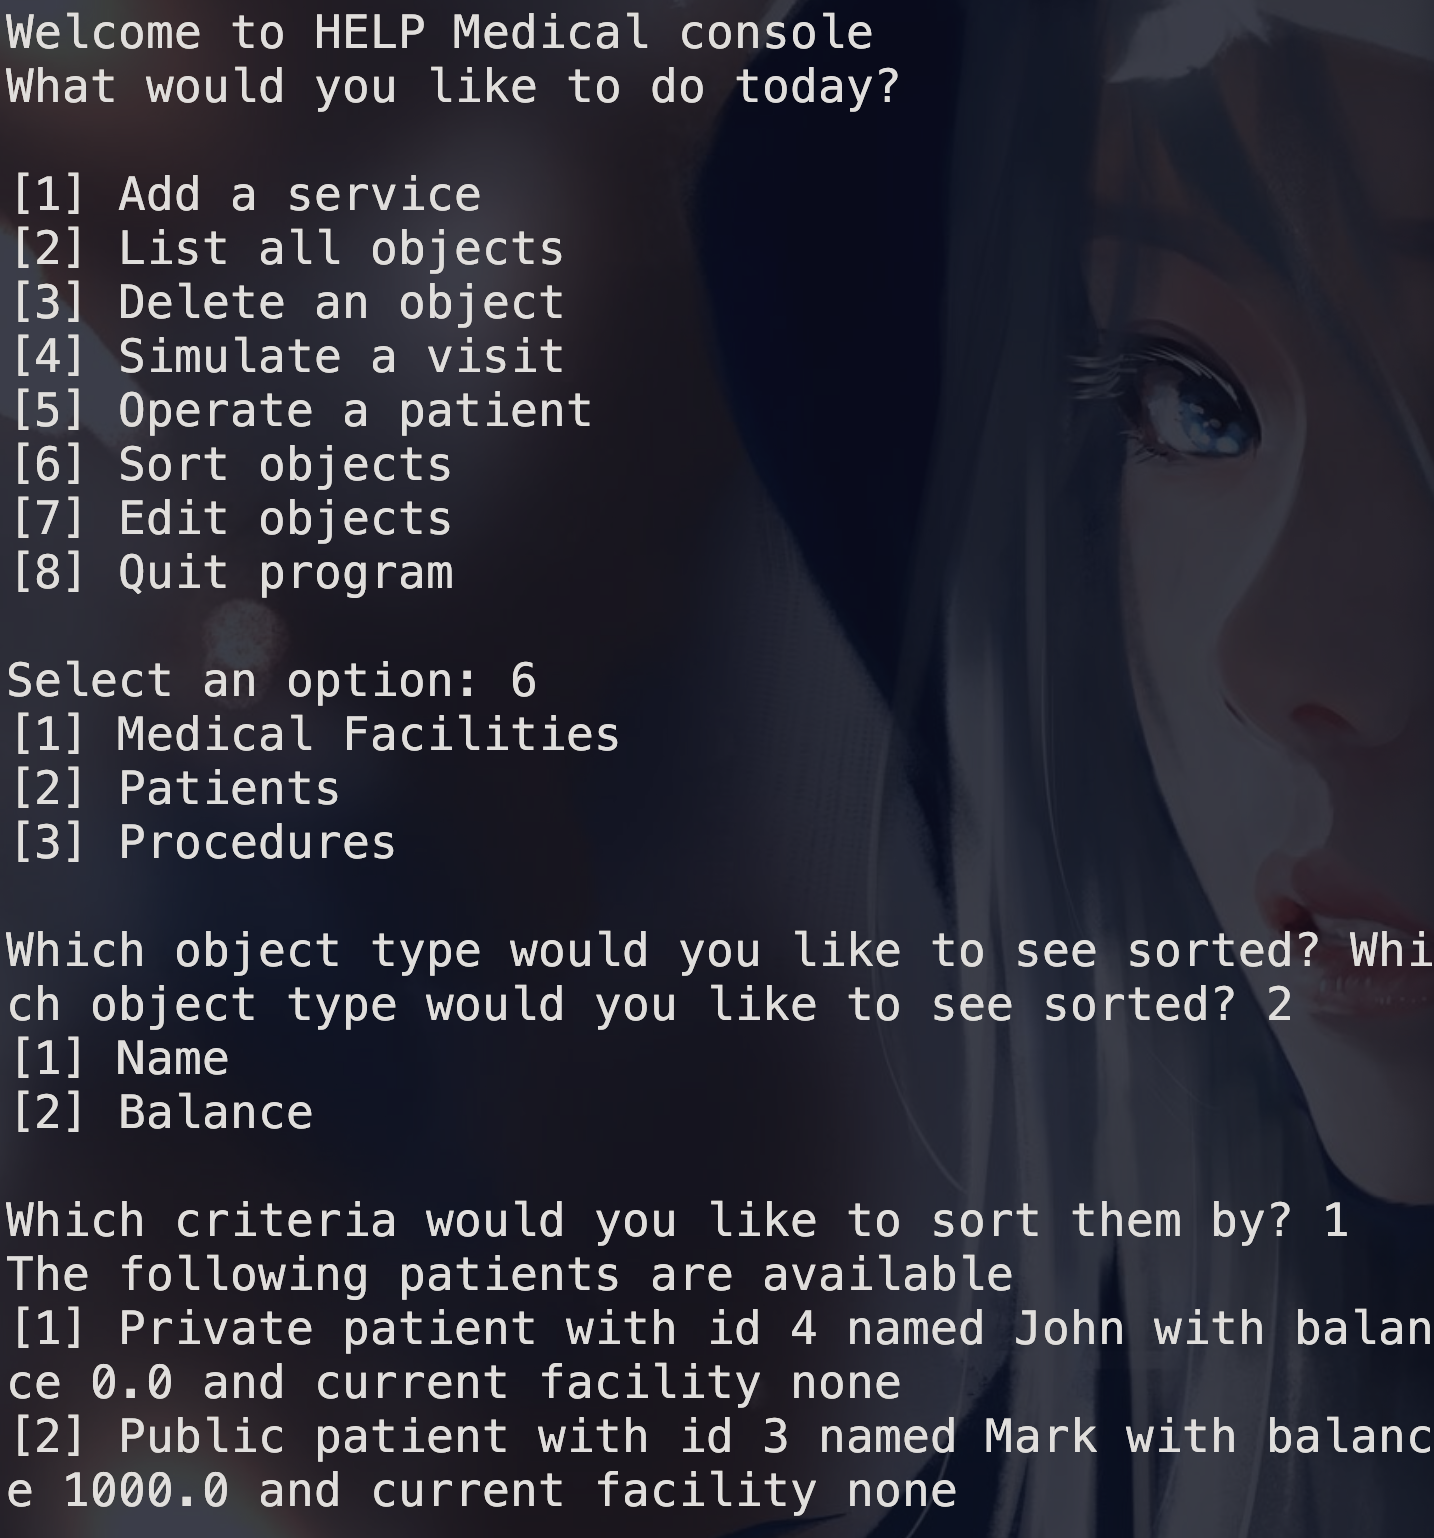
\includegraphics[width=0.6\textwidth]{figures/Sorting/Sorting_01.png}
		\end{center}
		\caption{Sorting patients by name}\label{fig:sorting_01}
	\end{figure}

	\begin{figure}
		\begin{center}
			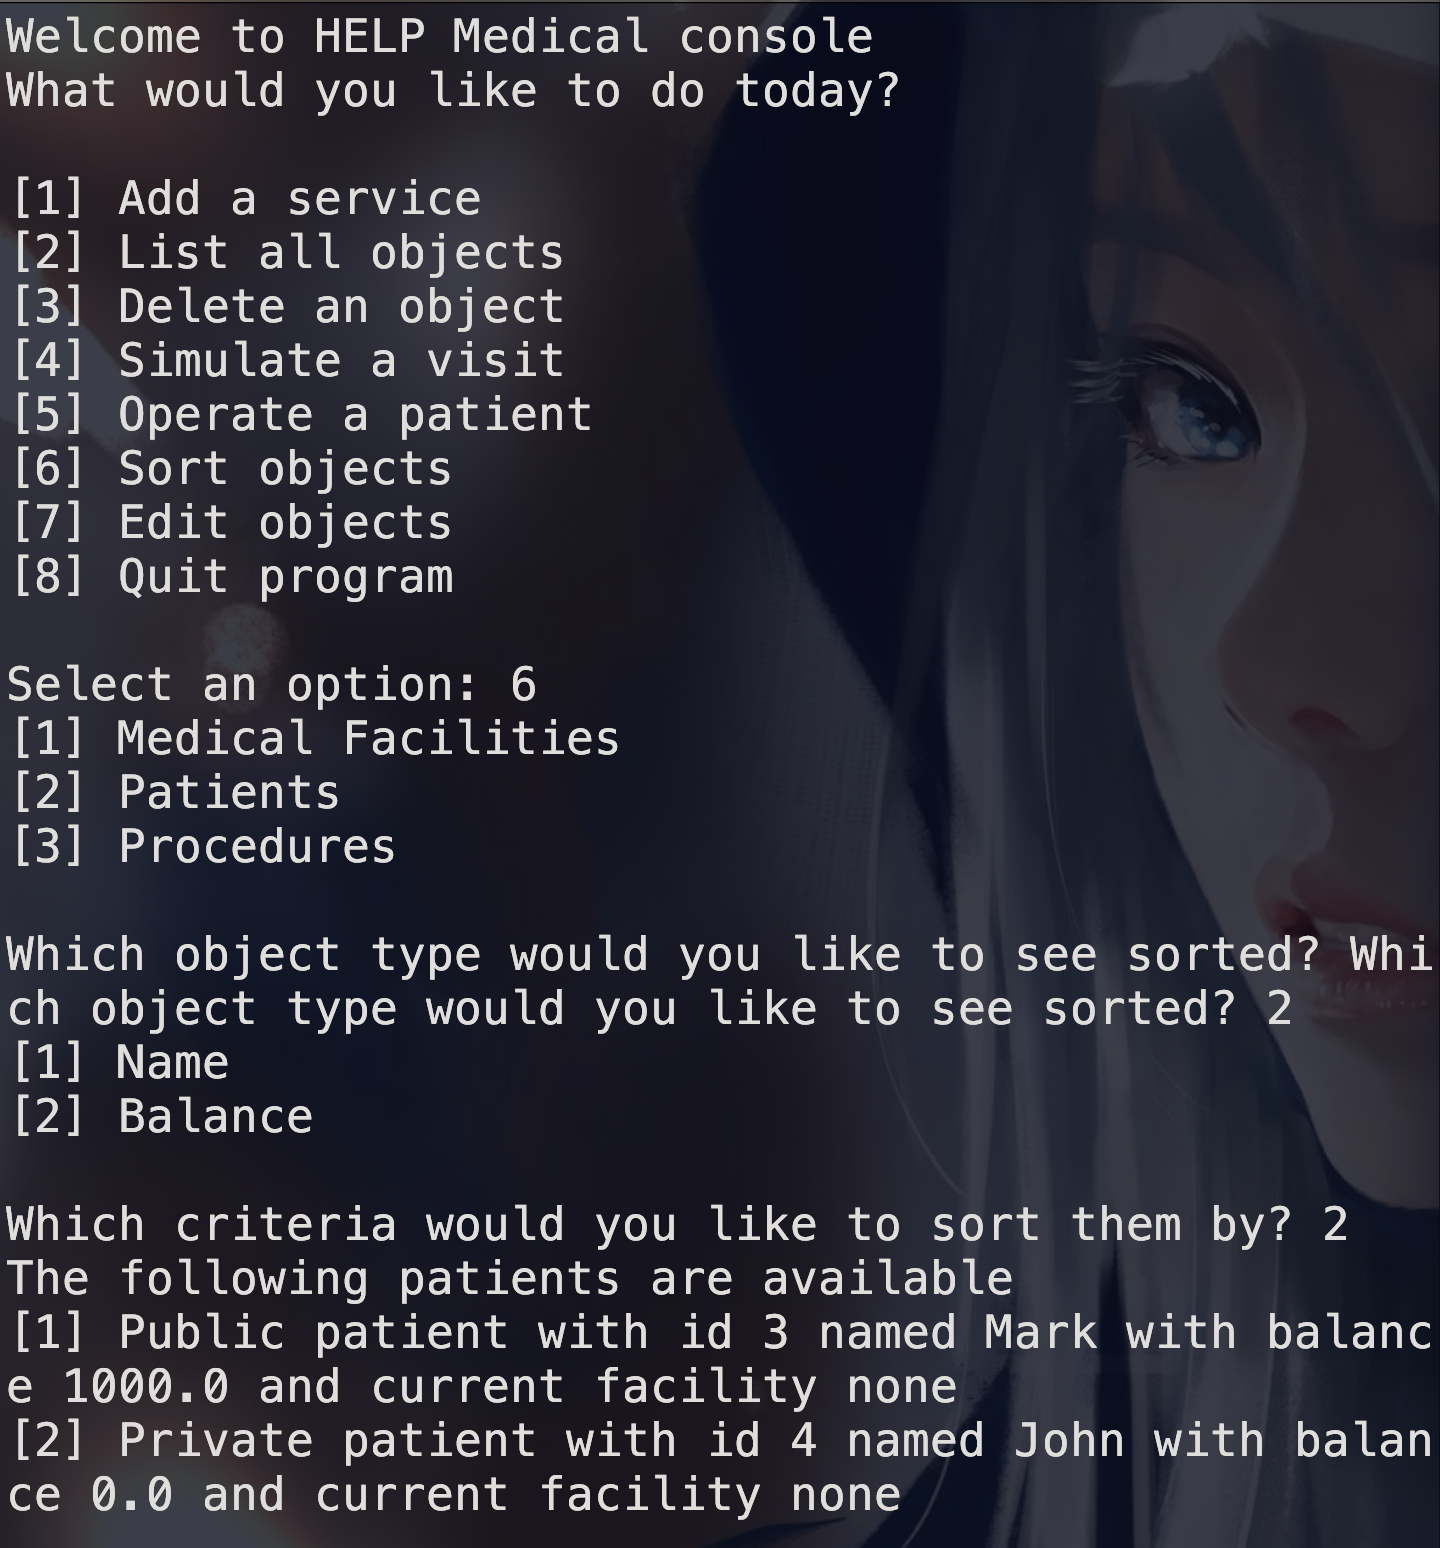
\includegraphics[width=0.5\textwidth]{figures/Sorting/Sorting_02.png}
		\end{center}
		\caption{Sorting patients by balance}\label{fig:sorting_02}
	\end{figure}
	% subsection Sorting objects (end)

	\subsection{Editing objects}\label{sub:editing_objects} % (fold)
	In this tests, the most complicated object in this program will be edited, that is a clinic. However, the flow of editing is generally the same. This application supports the editing of all fields, excluding non-primitive ones \ref{Editable}. For seeing all other editing methods being tested, please see \ref{Edit_tests}

	\begin{figure}
		\begin{center}
			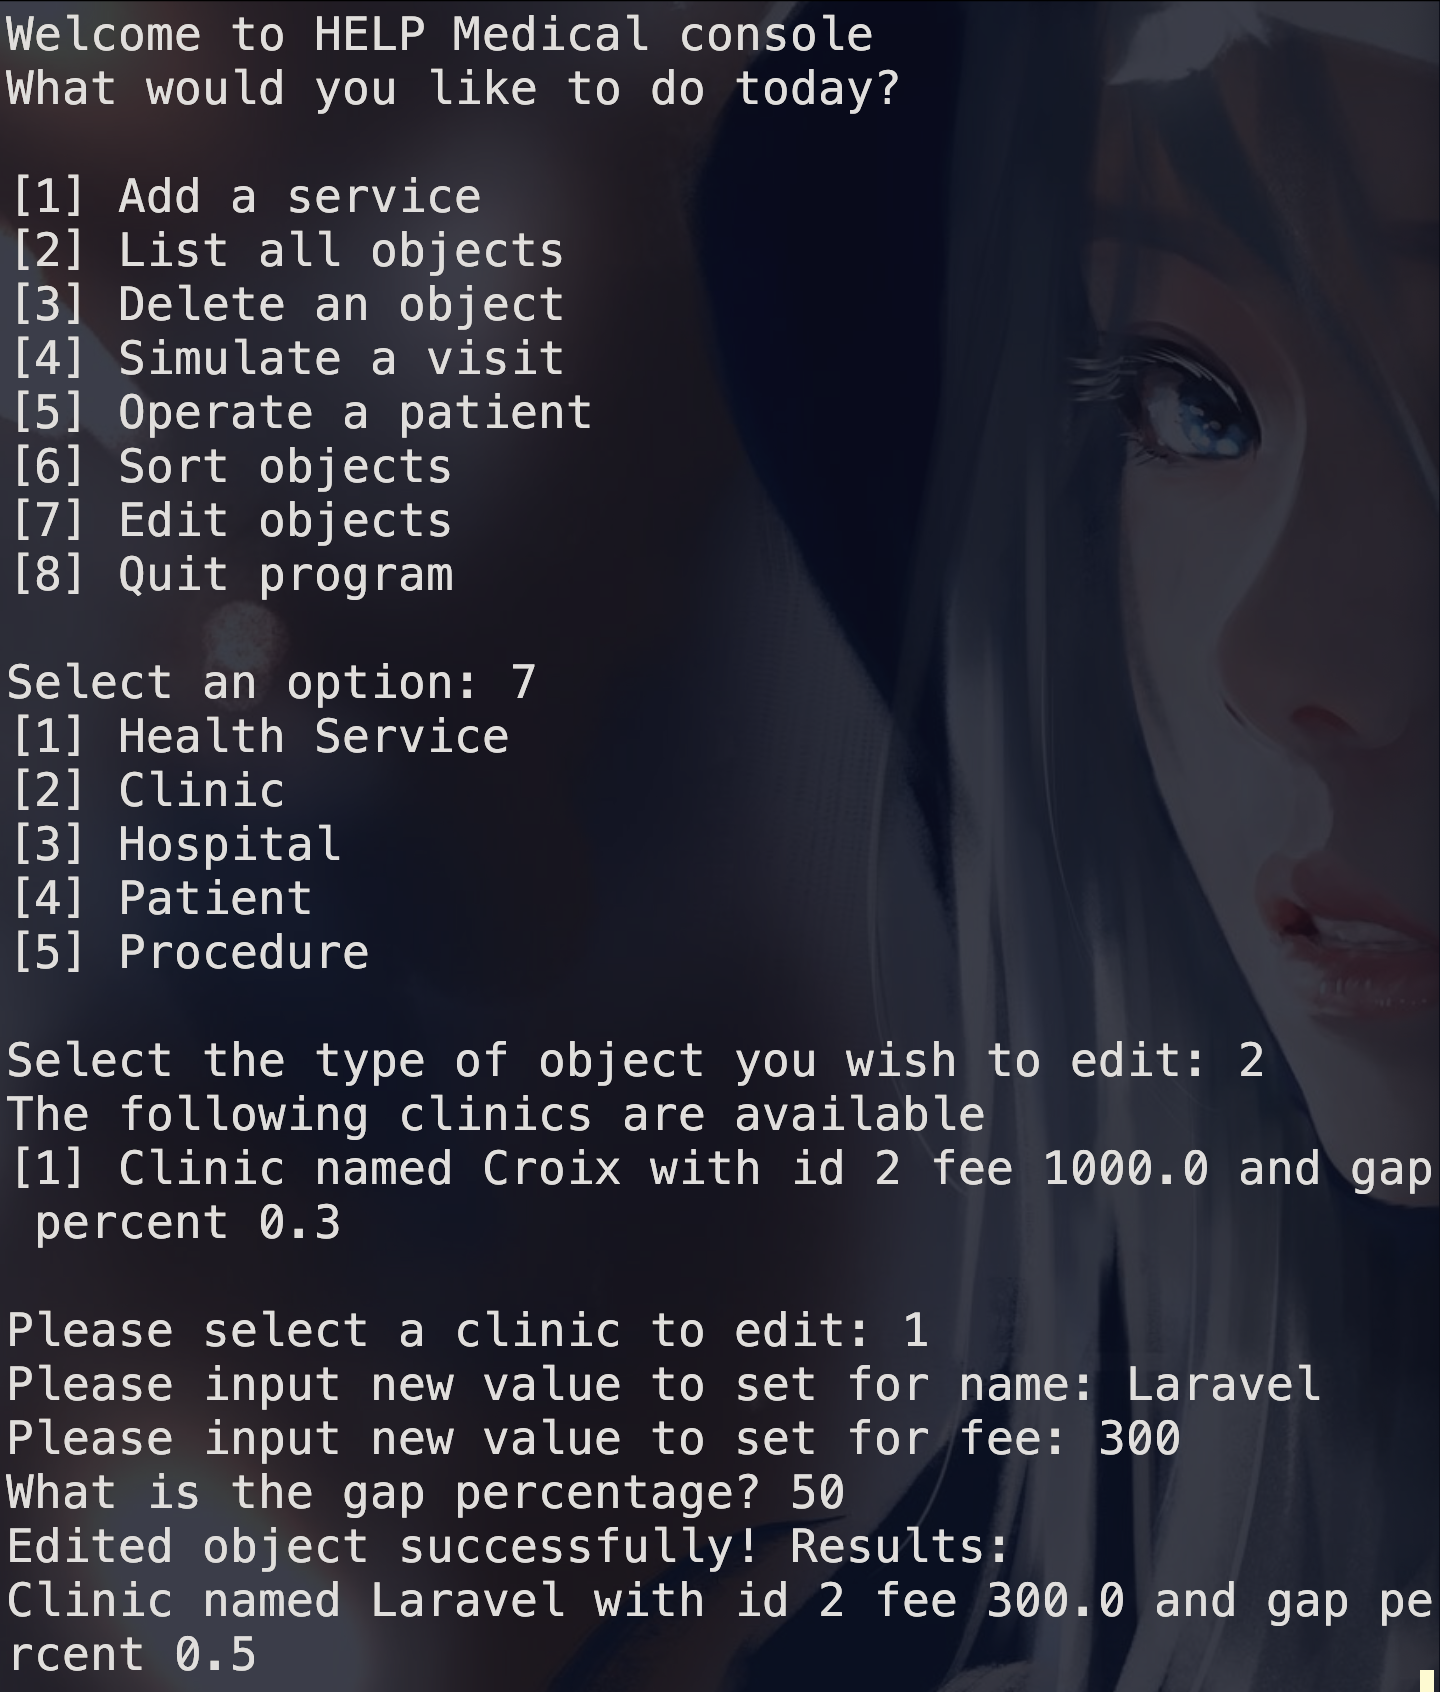
\includegraphics[width=0.6\textwidth]{figures/Editing/Editing_01.png}
		\end{center}
		\caption{Editing a clinic object}\label{fig:editing_01}
	\end{figure}

	As can be seen, the final output is correct, including the gap percentage, because the percentage set was $0.5$ although $50\%$ was input.
	% subsection Sorting objects (end)
	% section Extra features runtime output (end)

	\section{Bibliography}\label{sec:bibliography} % (fold)
	\printbibliography
	% section Bibliography (end)

\end{document}
